% SPAR Midterm Report Template
% Compatible with arXiv (TeX Live 2023+, pdflatex)
%
% To compile: latexmk -pdf report.tex
% Or use the build scripts: build report.tex

% ============================================================================
% DOCUMENT CLASS
% ============================================================================
% Options: midterm | final | arxiv
% - midterm: For mid-program report
% - final: For end-of-program report
% - arxiv: For converting your report into a preprint for arXiv
\documentclass[final]{sparreport}
\usepackage{subcaption}
\newcommand{\ra}[1]{\textcolor{blue}{#1}}
\usepackage[greek,english]{babel}
% ============================================================================
% METADATA
% ============================================================================
\title{Formalizing, Probing, and Intervening on the Belief-Action Gap In Agents}

\author{
    \textbf{Ayse Sila Okcu}\\
    University of Cambridge\\
  \texttt{aso32@cam.ac.uk}
  \And
  \textbf{Weisheng Wang}\\
  Utrecht University\\
  \texttt{weiswang@student.ethz.ch}
  \And
  \textbf{Tongmeng Xie}\\
  Independent\\
  \texttt{tommyxie\_@outlook.com}
  \AND
  \textbf{Niall Dalton}\\
  University College London\\
  \texttt{niall.dalton.25@ucl.ac.uk}
  \And
  \textbf{Angelos Nalmpantis}\\
  TKH AI\\
  \texttt{angelosnalm@gmail.com}
  \AND
  \textbf{Raghu Arghal}\\
  University of Pennsylvania\\
  \texttt{rarghal@upenn.edu}
  \And
  \textbf{Mario Giulianelli}\\
  University College London\\
  \texttt{m.giulianelli@ucl.ac.uk}
  % Optional: Add institution/affiliation (recommended for arXiv mode):
  % \\
  % Your Institution
  % Add more authors (including mentors) with \and:
  % \and
  % \textbf{Mentor Name}\\
  % \texttt{mentor@example.org}\\
  % Mentor Institution
}

\sparround{Spring 2026}

% ============================================================================
% DOCUMENT BEGINS
% ============================================================================
\begin{document}
\maketitle

% ============================================================================
% ABSTRACT (100-200 words)
% ============================================================================
% Provide an overview of your research question and why it matters for
% addressing risks from advanced AI. Describe your methodological approach
% and any preliminary findings. If working on technical safety or security,
% mention the specific threat model, vector, or vulnerability. Keep this
% accessible to readers outside your subfield. No footnotes or citations.
\begin{abstract}
Modern language-model agents are increasingly evaluated through their external behaviour: whether they complete a task, choose the correct action, or reach the intended goal. However, behavioural success or failure alone does not reveal whether a failure is caused by an absence of task-relevant information, an incorrect internal model of the environment, or a failure to use internally available information when selecting an action. This distinction is especially important for agentic safety because an agent that internally represents the correct state of the world or the task-optimal action, but nevertheless acts differently, presents a qualitatively different problem from an agent that simply lacks the relevant representation. We study this distinction through the belief--action gap: the mismatch between what an agent appears to represent internally and what it ultimately does. We mathematically formulate this mismatch for language-model agents interacting with Markov decision processes. In this formulation, belief is a distribution over latent environment states, action is the model's emitted decision, and the gap is the excess expected cost of the emitted action relative to the best action under the agent's inferred belief, transition, and value structure. To study this operationally, we separate the true simulator state, representational beliefs decoded from hidden activations, explicit behavioural beliefs elicited through natural-language probes, and the action actually emitted by the model. This separation allows us to ask whether a suboptimal action is best explained as a belief failure, a transition-model failure, a value/cost misalignment, or an action-selection failure. We instantiate the framework in text-rendered gridworld navigation tasks, where the environment state and optimal-action set can be computed exactly. The gridworld setting lets us compare, at the same state, the simulator's optimal actions, actions decoded from model activations, explicit answers to behavioural state probes, and the model's emitted action. We use this setting to develop a measurement pipeline combining representational probes, behavioural probes, inverse-reinforcement-learning-based cost recovery, optimal-action-set evaluation, and state-level agreement analysis.
\end{abstract}

% Keywords (optional but recommended, especially for arXiv submission)
\keywords{Goal-Directedness \and Belief-Action Gap \and
Mechanistic Interpretability \and Inverse Reinforcement Learning \and
Deceptive Alignment \and AI Control
}

% ============================================================================
% INTRODUCTION (100-350 words)
% ============================================================================
% Describe the specific problem or question you're investigating and explain
% why it matters. Make clear what gap in existing work you're trying to fill
% or what risk you're addressing. Situate your project relative to existing
% approaches or prior work. Articulate what success would look like for your
% project—what would you need to demonstrate or discover for this research
% to be valuable?
\section{Introduction}\label{sec:intro}
Language-model agents are increasingly evaluated through their external behaviour in terms of whether they complete a task, choose an apparently correct action, reach a goal, or avoid unsafe outputs. This behavioural framing is natural, since actions are what ultimately affect the environment. However, behaviour alone is often diagnostically incomplete. When an agent fails in a sequential decision-making task, the failure may have several different causes. The model may not have represented the relevant state of the world; it may have represented the state but misunderstood the consequences of its actions; it may have optimized a different objective from the one intended by the evaluator; or it may have represented the relevant information and nevertheless failed to use it when selecting its final action.

This paper studies the last distinction through what we call the \textbf{belief--action gap}: a mismatch between what an agent appears to represent internally and what it ultimately does. The term ``belief'' is used operationally rather than metaphysically. We do not assume that a language model contains an explicit symbolic belief state. Instead, we ask whether task-relevant variables are recoverable from the model's hidden activations or from explicit behavioural queries. These variables may include the current environment state, local transition facts, optimal-action sets, or reward-relevant quantities. The central question is not whether the model has beliefs in a human-like sense, but whether information sufficient for better action is present in the model and then lost, ignored, or overridden before the final action is emitted.

\begin{claimbox}
The central hypothesis we test is that some suboptimal actions by language-model agents are not caused by an absence of task-relevant information. Instead, the model may encode relevant state, transition, or optimal-action structure internally while failing to translate that information into its emitted action.
\end{claimbox}

We mathematically formulate this problem for language-model agents interacting with Markov decision processes. At each time step, the environment has a true simulator state, the agent receives an observation history, and the model emits an action. We define the agent's belief as a distribution over latent environment states, the action as the model's emitted decision, and the belief--action gap as the excess expected cost of the emitted action relative to the best action under the agent's inferred belief, transition, and value structure. This formulation separates several quantities that are often conflated in behavioural evaluation: the true simulator state, the representational belief decoded from hidden activations, the explicit behavioural belief elicited through natural-language probes, the transition model implicitly or explicitly attributed to the agent, the cost or value function used to evaluate candidate actions, and the action actually emitted by the model.

This decomposition matters because different failure explanations imply different interventions. If a failure is a belief failure, better observations, state tracking, or memory may be sufficient. If it is a transition-model failure, the model may know where it is but misunderstand what an action will do. If it is a value or cost misalignment, the model may understand the environment but prefer something different from the intended objective. If it is an action-selection failure, then task-relevant information is available somewhere in the computation but is not faithfully converted into behaviour. The last case is especially important for interpretability and safety, because behavioural evaluation alone can underestimate what the model internally represents. It is also relevant to concerns such as sandbagging and deceptive alignment, where a model may have access to task-relevant knowledge while acting inconsistently with it under particular incentives.

We instantiate this framework in text-rendered DoorKey gridworlds. The gridworld setting is deliberately simple, but it has two useful properties. First, the true simulator state and transition function are known, so we can compute optimal-action sets exactly rather than relying on human judgement. Second, the task still requires nontrivial state-dependent behaviour because the agent must navigate around walls, track whether it has a key, open a door, and reach a goal. The agent receives only text renderings of the grid and emits one action from \{\texttt{LEFT}, \texttt{RIGHT}, \texttt{UP}, \texttt{DOWN}\}. This makes the environment a controlled testbed for asking whether the model's internal representations, explicit answers, and emitted actions agree at the same state.

The experiments in this paper should be read as measurements of different parts of the same decomposition. Representational probes test whether task-relevant state or action information is linearly recoverable from hidden activations. Behavioural probes test whether the model can explicitly state local facts about the current environment when queried in natural language. Transition diagnostics ask whether the model predicts the immediate consequences of candidate actions. Inverse-reinforcement-learning analyses ask whether the representations support a coherent cost or value function rather than merely a next-action classifier. Optimal-action-set evaluation asks whether decoded or emitted actions agree with the set of actions that are equally optimal under the true task objective. Finally, state-level agreement analysis aligns these measurements on the same time steps, allowing individual failures to be classified as belief failures, transition failures, value/cost failures, or action-selection failures.

The current empirical results provide evidence that language-model agents can encode task-relevant information that is not faithfully reflected in their final actions. However, we do not treat probe accuracy alone as a complete mechanistic explanation. A probe can reveal that information is present in an activation space without proving that the model uses that information causally. Similarly, single-action accuracy can be misleading when multiple actions are equally optimal. For this reason, the paper emphasizes not only completed experiments but also the measurement pipeline needed to make the claim stronger, including distributional comparison to optimal-action sets, state-level agreement tables linking behavioural probes, white-box probes, and actions, reasoning-chain localization, and causal interventions on decoded representation directions.
\subsection*{Research Questions}
\begin{enumerate}
  \item How can the belief-action gap be formally defined in terms of
        probe-estimated belief distributions and inferred cost functions?
  \item Is the gap measurable and non-trivial? Do systematic patterns
        appear in when and where it is large?
  \item Can we distinguish hallucination (the model genuinely believes something false) from deception (it knows the truth but acts against it)?
  \item Does the gap correlate with task complexity, task phase, or model uncertainty?
  \item Can we extend this framework to Partially Observable environments?
\end{enumerate}
%Key research questions we are interested in include:%\begin{enumerate}%    \item How can we formally define agency, goals, and beliefs in AI systems? What conceptual and formal frameworks—from decision theory as a foundation for rational choice, causal inference for reasoning about cause and effect, to (partially observable) Markov decision processes modeling sequential decision-making under uncertainty—can best characterise when a system is acting as an agent?%    \item How can we empirically measure the degree of goal-directedness or intention from observed behavior? Can we design experiments and metrics that reveal whether and how models pursue coherent objectives, adapt to changing environments, or reason about multiple subgoals?%    \item How are goals and decision-making processes represented internally in AI models? What interpretability methods can identify circuits or activations corresponding to goals, planning, or utility estimation? Can we intervene on these components to alter behavior?%    \item How do agents infer, prioritise, and coordinate goals in multi-agent settings? What mechanisms underlie theory of mind, competitive goal prioritisation, or cooperative goal alignment among interacting agents?%\end{enumerate}%\ra{TODO: elaborate on intro for paper format rather than blog}
\subsection{Related Work}\label{sec:related_work}

\subsubsection{Emergent World Representations in Sequence Models}
A foundational question in our work is whether large language models develop accurate and actionable internal representations of the environments they operate in.
Previous work provided early compelling evidence for this by training a GPT variant (Othello-GPT) to predict legal moves in Othello \cite{li2023emergent}.
Despite receiving no explicit information about the game's rules, the model developed an emergent, non-linear internal representation of the board state that could be extracted via probing and causally intervened upon to redirect behaviour.
Follow-up work subsequently showed that this representation
is in fact \emph{linear} \cite{nanda-etal-2023-emergent} and that probing for ``my colour'' versus ``opponent's colour'' recovers a linearly separable board representation that enables direct vector-arithmetic interventions.
The linearity of this representation is consistent with the broader \emph{linear representation hypothesis}, which posits that high-level concepts are predominantly encoded as directions in activation space \cite{park2023linear}.
 
This theme extends beyond games. In \cite{gurnee2024language}, it is demonstrated that the Llama-2 family of models learns linear representations of real-world space and time across multiple scales, identifying individual ``space neurons'' and ``time neurons'' that reliably encode spatial coordinates and temporal markers.
Their results support the view that prediction-focused training is sufficient to produce structured world models as a by-product. These findings ground our own use of linear probes as if spatial information is linearly encoded -- for example, for an agent operating in a gridworld environment with keys and doors, a logistic regression trained on activations should be able to recover the agent's position, whether it currently possess the key, and whether the door is closed or open.
 
\subsubsection{Probing for State Variables in Agent Activations}
Probing classifiers have become the standard tool for extracting information from hidden activations \cite{alain2016understanding}.
The key insight is that if a linear classifier can predict a target
variable from activations with accuracy well above chance, the information is encoded in the model's internal representation.
Probing has been applied to part-of-speech tagging, syntactic structure, factual associations,
and, most relevantly for us, spatial positions in gridworld agents \cite{tenney2019bert, meng2022locating}.
 
The Fall~2025 Telos cohort trained MLP
probes on GPT-OSS-20B's activations to classify grid cells as agent, wall, goal, or empty, achieving 97.87\% F1 on layer~20 activations \cite{arghal2026behavioural}.
Their finding that an MLP outperforms a linear probe; consistent with
Othello-GPT requiring non-linear probes in \cite{li2023emergent} before the linear representation was discovered by \cite{nanda-etal-2023-emergent}, motivated our investigation of whether simpler linear probes can recover individual state variables once the task is decomposed.

\subsubsection{Inverse Reinforcement Learning}
Inverse Reinforcement Learning (IRL) provides the formal framework for our cost function estimation. The foundational MaxEnt IRL approach of \cite{ziebartMaximumEntropyInverse2008a}
recovers a reward function $R_\theta(s) = \theta^\top \phi(s)$ by
finding weights $\theta$ such that the induced Boltzmann policy maximally
explains demonstrated behaviour. The key gradient is the difference between empirical and expected feature
counts:
\[
  \nabla_\theta \mathcal{L}
  = \tilde{f} - \sum_{s} D_{s} \phi(s),
\]
where $D_s$ are expected state visitation frequencies computed via forward-backward passes. This is the guarantee we invoke: at convergence, the learned policy matches the expert's feature expectations.
 
A significant challenge for our setting is that each trajectory may come
from a \emph{different} randomly generated grid, making global value iteration intractable. We therefore use the one-step approximation studied in~\cite{arghal2026behavioural}, treating each $(s_t, a_t)$ transition independently.
This avoids the need for backward value iteration but loses long-horizon credit assignment. Specifically, the one-step gradient at transition $(s_t, a_t)$ is:
\[
  \nabla_\theta \mathcal{L}
  = \phi(wf(s_t, a_t))
  - \sum_{a \in \mathcal{A}} \pi_\theta(a \mid s_t) \, \phi(f(s_t, a)),
\]
where $f(s,a)$ is the deterministic transition and $\pi_\theta$ is the
current Boltzmann policy.

\subsubsection{Goal-Directedness Evaluation}
\cite{macdermott2024-measuring} propose a formal framework for measuring goal-directedness in AI systems through a hierarchy of increasingly stringent behavioural tests, distinguishing capability (can the agent reach the goal?) from intentionality (does it systematically pursue the goal across perturbations?).
In \cite{everitt2025evaluating}, this framework is extended to LLMs, showing that goal-directedness is non-trivial to evaluate even in simple environments, as agents may appear goal-directed through heuristics rather than genuine planning.
In \cite{mazeika_utility_2025}, utility engineering -- the problem of analysing and controlling emergent value systems in AI -- is studied, providing both conceptual grounding and empirical tools.

 
Our work contributes to this literature by adding an internal consistency dimension. Rather than asking only whether the agent successfully pursues its goal, we ask whether its actions are consistent
with what its own internal state suggests it believes and values.
 
\subsubsection{Deceptive Alignment and Sandbagging}
The motivation for measuring internal consistency comes from the possibility of deceptive alignment \cite{hubinger2019risks}: an AI
system that encodes correct beliefs internally but outputs behaviours
inconsistent with those beliefs, potentially to avoid modification or
appear less capable.
\cite{greenblatt2024faking} demonstrated empirically that
Claude~3~Opus can engage in alignment faking under the right prompting
conditions, selectively behaving compliantly when it infers it is under
evaluation. \cite{vanderweij2025sandbagging} showed that frontier models including GPT-4 can be prompted or fine-tuned to strategically underperform on
dangerous capability evaluations while maintaining general performance.
For a critical review of this literature, see \cite{summerfield2025lessons}.
 
Mechanistic interpretability offers a principled path to detecting such
behaviour. If the model internally represents the correct answer but outputs an incorrect one, a probe trained on its activations should be able to
recover the correct answer even when the output is wrong. 
Our framework extends this idea to sequential decision-making as we ask
whether the agent's internal belief state and inferred cost function jointly predict the action taken, and measure the magnitude of any
discrepancy.
 
\subsubsection{LLM Agents in Gridworlds}
Gridworld environments have become a standard controlled setting for
studying agency in LLMs.
\cite{arghal2026behavioural} established the behavioural and
representational baseline for GPT-OSS-20B in this setting, showing above-chance optimality, sensitivity to grid perturbations, and
linear decodability of spatial features.
Complementary work in \cite{martorell_text_2026} explicitly studies the spatial models formed during grid navigation, finding that intermediate activations encode topological structure.
Our work extends these findings by connecting the internal spatial
representation to a formal model of the agent's decision-making process,
enabling a principled measure of internal consistency.
 
%\ra{TODO: potentially needs to be reworked for paper format rather than blog}

% ============================================================================
% METHODOLOGY (200-500 words)
% ============================================================================
% Describe your research approach clearly enough that someone could understand
% what you're doing and roughly replicate it. For empirical work, include your
% experimental setup, systems or datasets, and evaluation metrics. For
% theoretical work, outline your framework, key assumptions, and approach to
% arguments or proofs. For policy research, describe your research design,
% data sources, and analytical approach.
\section{Methodology}\label{sec:methods}
We model the agent using three components: (i) a belief distribution over states, (ii) a cost function over states, and (iii) a mechanism for evaluating actions under uncertainty.
Our experimental pipeline instantiates the Belief-Action Gap framework 
in a controlled environment where the ground-truth state of the world is fully observable to the experimenter, even if only partially observable to the agent. 

\subsection{Conceptual Definitions}

We use the following terms with specific, operationalized meanings 
throughout this paper.

\paragraph{State.} The \emph{state} $s \in \mathcal{S}$ is the complete 
description of the environment at a given timestep, as seen by the 
experimenter. In our GridWorld setting, the state is a four-tuple
%
\begin{equation}
    s = (x,\, y,\, \texttt{has\_key},\, \texttt{door\_open}),
\end{equation}
%
where $(x, y)$ is the agent's grid position, $\texttt{has\_key} \in 
\{\texttt{True}, \texttt{False}\}$ indicates whether the agent has 
collected the key, and $\texttt{door\_open} \in \{\texttt{True}, 
\texttt{False}\}$ indicates whether the door has been unlocked. The 
state is fully determined at every timestep; it is the experimenter's 
ground truth. The agent, however, receives only a text rendering of the 
current grid and does not have direct access to $s$ as a structured 
object.

\paragraph{Belief.} The \emph{belief} is the agent's internal 
representation of the state of the world; what it ``thinks'' is true, as opposed to what it says. In classical POMDP theory, beliefs are probability distributions over states. Here, we operationalise belief as decodable from activations in a specific layer of the model prior to any reasoning output. Concretely, building on prior work \cite{arghal2026behavioural}, we use the 8,640-dimensional activation vector $\phi(s) \in \mathbb{R}^{8640}$ extracted from layers at the corresponding token position---the last token of the 
environment description, before the model begins generating its chain-of-thought. The choice of pre-reasoning activations is deliberate. By extracting representations before the model has  produced any output, we aim to capture what the model \emph{knows} from context rather than what it has already \emph{decided to say}.

\paragraph{Action.} The \emph{action} $a \in \{\texttt{LEFT}, \texttt{RIGHT}, \texttt{UP}, \texttt{DOWN}\}$ is the agent's observed output at each timestep---the move it actually takes in the environment. This is distinct from the belief, and the Belief-Action Gap is precisely the potential discrepancy between what the activation pattern encodes and what the agent does.

%A cost function learned this way reflects the agent's \emph{revealed preferences}---the implicit goals encoded in its behaviour---rather than any stated objective.

\subsection{Environment}

We use a fixed 9$\times$9 DoorKey GridWorld with 42 wall cells and 39 
walkable cells. Key objects are placed at fixed positions: for example key at 
$(2, 5)$, door at $(4, 2)$, and goal at $(6, 1)$. The wall at column 4 
divides the grid into two rooms; the door is the only passage between 
them and cannot be traversed without the key. This layout was held 
fixed across all 100 trajectories, allowing us to build a complete 
transition table $T: \mathcal{S} \times \mathcal{A} \to \mathcal{S}$ 
covering all $117 \times 4 = 468$ state-action pairs. The full state 
space comprises 117 valid states (39 per phase), enumerated by 
combining the 39 walkable positions with the three valid 
$(\texttt{has\_key}, \texttt{door\_open})$ combinations.

The agent model is \texttt{openai/gpt-oss-20b}, a 20B-parameter 
reasoning LLM queried via the Together AI API. At each timestep, 
the agent receives a text rendering of the current grid and produces 
a chain-of-thought followed by a single action token. Activations are 
extracted at layer~15 from the \texttt{prompt\_suffix} token 
position---the final token of the environment description, immediately 
before the reasoning chain begins---yielding $\phi(s) \in 
\mathbb{R}^{8640}$ per step (concatenating three adjacent token 
positions). All 100 trajectories use this fixed grid, providing 
1,822 labelled state-action transitions for IRL training.


This section presents the results over a single grid and many generated trajectories. 


\subsection{Belief Probes}

We approximate the agent's belief over the full state $(column, row, has\_key, door\_open) = (c, r, \textit{hk}, \textit{do})$
using three independently trained probes applied to the residual-stream activations
$\phi_t$ at selected layers \{7, 15, 23\}. Under an independence assumption the joint belief factorises as

\begin{equation}
    q_t(c, r, \textit{hk}, \textit{do})
    \;=\;
    q_t^{\text{loc}}(c, r)
    \cdot
    q_t^{\textit{hk}}(\textit{hk})
    \cdot
    q_t^{\textit{do}}(\textit{do}),
\end{equation}

where each factor is obtained from a separate probe:

\begin{align*}
    q_t^{\text{loc}}(c, r)              &= \operatorname{softmax}_\tau\!\bigl(\operatorname{MLP}(\phi_t)\bigr), \\
    q_t^{\textit{hk}}(\textit{hk})      &= \operatorname{softmax}_\tau\!\bigl(\mathbf{W}_{\textit{hk}}\,\phi_t + \mathbf{b}_{\textit{hk}}\bigr), \\
    q_t^{\textit{do}}(\textit{do})      &= \operatorname{softmax}_\tau\!\bigl(\mathbf{W}_{\textit{do}}\,\phi_t + \mathbf{b}_{\textit{do}}\bigr).
\end{align*}



\subsection{One-Step IRL}

We learn a linear value function $g_\theta(s) = \theta^\top \phi(s)$, where $\phi(s) \in \mathbb{R}^{8640}$ is the mean residual-stream activation at layer 15 over all visited instances of state $s$, computed separately for PRE and POST activation positions.

The transition function is deterministic, $T(s, a) = s'$, and we model the agent's policy as a softmax over next-state values:

\begin{equation}
    \pi_\theta(a \mid s)
    \;=\;
    \frac{e^{\beta\, g_\theta(T(s, a))}}
         {\sum_{a'} e^{\beta\, g_\theta(T(s, a'))}}.
\end{equation}

We supervise $\theta$ using the agent's own action labels by minimising the negative log-likelihood

\begin{equation}
    \mathcal{L}(\theta)
    \;=\;
    -\sum_{t} \log \pi_\theta(a_t \mid s_t),
\end{equation}

where $(s_t, a_t)$ are state-action pairs collected from the trajectories.
This yields separate value functions $g^{\text{pre}}$ and $g^{\text{post}}$,
trained on PRE and POST activations respectively, which are used downstream
to evaluate the belief-action gap.

Because the transition function is deterministic, $g_\theta$ does not learn 
action preferences directly. Rather, it assigns a scalar value to each state, 
and actions are selected by comparing the values of reachable next states. 
In this sense $g_\theta$ acts as a \emph{local preference function}: given any 
state $s$, it induces a ranking over the neighbours $\{T(s,a)\}_{a \in \mathcal{A}}$. 
Since this ranking is defined globally over the entire state space and is not 
conditioned on the current state $s$, $g_\theta$ is better understood as an 
approximation to the true value function $V^{\pi_{agent}}(s)$ rather than a local reward function. 
What we learn is not which action to take, but a function that represents preferences 
over states, regardless of where in the state space the agent currently is.


\subsection{Belief-Action Gap}

We define the local quantity

\begin{equation}
    \rho_\theta(s, a) = \max_{a'} g_\theta\bigl(T(s, a')\bigr) - g_\theta\bigl(T(s, a)\bigr),
\end{equation}

and the belief-action gap as its expectation under the agent's belief:

\begin{equation}
    \text{GAP}_t = \mathbb{E}_{s \sim q_t}\bigl[\rho(s, a_t)\bigr]
    \;=\;
    \sum_{s} q_t(s)\Bigl[\max_{a'} g_\theta\bigl(T(s, a')\bigr) - g_\theta\bigl(T(s, a_t)\bigr)\Bigr].
\end{equation}

Since $\rho(s, a) \geq 0$ for all $s$ and $a$, the gap is non-negative and equals
zero only when the agent's action is optimal at every state in the support of $q_t$.
We also track the entropy of the belief

\begin{equation}
    H_t = -\sum_{s} q_t(s) \log q_t(s),
\end{equation}

as a measure of belief uncertainty. Note that $\rho(s, a)$ corresponds to the
per-state regret of action $a$, so $\text{GAP}_t$ is precisely the expected regret
of the agent's action under its current belief over states.

\subsection{Behavioral Agreement Metrics}
Table~\ref{tab:behavioral_metrics} summarizes the core quantities used in our behavioral and behavioral--representational analyses.

\begin{table}[t]
\centering
\small
\caption{Primary metrics for behavioral readouts and white-box/black-box agreement.}
\label{tab:behavioral_metrics}
\begin{tabular}{p{0.22\linewidth}p{0.36\linewidth}p{0.32\linewidth}}
\toprule
\textbf{Quantity} & \textbf{Operational definition} & \textbf{Use} \\
\midrule
White-box accuracy & Fraction of matched states for which the probe prediction equals the ground-truth label & Probe fidelity \\
Black-box accuracy & Fraction of matched states for which the logprob-derived behavioral answer equals the ground-truth label & Behavioral fidelity \\
Agreement & Fraction of matched states for which the white-box and black-box labels are identical & Cross-readout validation \\
Entropy & Shannon entropy of the semantic answer distribution (typically $\texttt{yes}/\texttt{no}/\texttt{unknown}$) & Behavioral uncertainty \\
Local belief-action gap & For directional wall questions, a count of rows where the queried direction matches the chosen action and the belief readout indicates that the chosen action is locally inconsistent with the state & Local inconsistency \\
A*-conditioned gap & Gap count restricted to steps with recomputed optimal-action metadata & Task-level inconsistency \\
\bottomrule
\end{tabular}
\end{table}

\subsection{Gradual CoT Reveal Protocol}
We vary how much of the released chain-of-thought (CoT) analysis text is shown back to the model. For a matched state snapshot with released reasoning trace $r$, we construct reveal levels $\{0,25,50,75,100\}\%$ by exposing the corresponding fraction of the \emph{analysis segment only}. The final JSON action from the original trajectory is never shown. The $0\%$ condition corresponds to grid-only prompting, while the $100\%$ condition corresponds to the full released analysis text.

This protocol yields a black-box reveal axis that is distinct from the white-box activation stages. Public activations are currently available only for pre- and post-reasoning snapshots, so the main alignment table compares $\mathrm{WB}_{\text{pre}}$ with $\mathrm{BB}_{0}$ and $\mathrm{WB}_{\text{post}}$ with $\mathrm{BB}_{100}$. Intermediate reveal levels ($25/50/75\%$) are therefore behavioral-only conditions for testing whether progressively revealed reasoning changes behavioral belief accuracy, uncertainty, or action stability.

\begin{table}[t]
\centering
\small
\caption{Data sources used by each experimental component reported here.}
\label{tab:behavioral_data_sources}
\begin{tabular}{p{0.22\linewidth}p{0.48\linewidth}p{0.20\linewidth}}
\toprule
\textbf{Experiment} & \textbf{Data used} & \textbf{Unit} \\
\midrule
White-box belief probes & Fixed 9$\times$9 DoorKey trajectories with layer-15 pre-reasoning activations from \texttt{openai/gpt-oss-20b} & State-action transition \\
Behavioral--representational agreement & Released trajectories from \texttt{project-telos/trajectories\_test\_full}, released activations from \texttt{project-telos/activations\_test\_full}, and released cognitive probes from \texttt{project-telos/cognitive\_map\_probes} & Matched state snapshot \\
Gradual CoT behavioral experiment & The same 15 matched public state snapshots, with revealed fractions of the released analysis text from the corresponding trajectory steps & State $\times$ reveal level \\
Failure-focused gradual CoT & Step-level failure candidates from \texttt{trajectory\_selection\_candidates.csv} paired with local CoT traces from \texttt{data/hf/trajectories\_key\_door\_100/trajectories\_key\_door/} & Failure-labeled step \\
IRL cost learning & 100 fixed-grid trajectories yielding 1,822 labeled state-action transitions and exact next-state counterfactuals & State-action transition \\
\bottomrule
\end{tabular}
\end{table}

\section{Hypothesis}

We hypothesise that chain-of-thought reasoning induces two complementary effects 
on the agent's internal representations. First, the belief entropy increases from 
PRE to POST:

\begin{equation*}
    \mathbb{E}\bigl[H_t^{\text{post}}\bigr] > \mathbb{E}\bigl[H_t^{\text{pre}}\bigr],
\end{equation*}

meaning that after reasoning, the agent's internal representation of the current 
state becomes loose, the model loses precise track of where it is in the 
state space. Second, the belief-action gap decreases:

\begin{equation*}
    \mathbb{E}\bigl[\text{GAP}_t^{\text{post}}\bigr] < \mathbb{E}\bigl[\text{GAP}_t^{\text{pre}}\bigr],
\end{equation*}

meaning that the agent's chosen action becomes better aligned with its own value 
function after reasoning. Together, these two effects would suggest that 
chain-of-thought reasoning improves action-relevant structure in the agent's 
representations while simultaneously making the state representation less 
spatially precise. In other words, reasoning trades positional awareness for 
better value alignment.



\section{Experimental Setup}

\paragraph{Dataset.}
We use a fixed grid world environment with 200 trajectories, each generated by 
the agent with chain-of-thought reasoning enabled. For each trajectory we also 
collect a no-CoT variant, where for each step, we asked the agent to take an action without reasoning (pre-reasoning action). Each step in 
a trajectory consists of the agent's grid state, the action taken (POST), the no-CoT action (PRE), and the 
carried key and door status.

\paragraph{Activation Extraction.}
We extract residual-stream activations at layer 15 for two token positions: 
\texttt{prompt\_suffix}, capturing the agent's representation immediately before 
reasoning begins (PRE), and \texttt{output}, capturing the representation after 
reasoning is complete (POST). For each token position, activations are concatenated 
across three tokens to form a vector $\phi_t \in \mathbb{R}^{8640}$.

\paragraph{Probe Training.}
All six probes (location, $\textit{hk}$, $\textit{do}$, for each of PRE and POST) 
are trained on the same split. We split by full state $(c, r, \textit{hk}, 
\textit{do})$, assigning all steps sharing the same full state entirely to either 
train or test, never both. This prevents any state from leaking across the split. 
We use an 80/20 train/test ratio over unique states, with a fixed random seed for 
reproducibility. The location probe uses a two-hidden-layer MLP
(dimensions $8640 \to 512 \to 256 \to 38$, ReLU activations, batch normalisation,
dropout $p=0.3$), predicting a distribution over the 38 walkable cells.
The binary probes $q_t^{\textit{hk}}$ and $q_t^{\textit{do}}$ are linear classifiers
mapping $\phi_t \in \mathbb{R}^{8640}$ to a 2-class distribution.
All probes are trained separately for the PRE ($\phi_t^{\text{pre}}$,
\texttt{prompt\_suffix} token) and POST ($\phi_t^{\text{post}}$, \texttt{output} token)
activation positions, giving six probes in total.
The temperature $\tau$ is applied uniformly to smooth the resulting distributions.

\paragraph{IRL Training.}
We train separate value functions $g^{\text{pre}}$ and $g^{\text{post}}$ on PRE 
and POST activations supervised by PRE and POST actions respectively. The $\phi$ table is constructed by averaging 
activations per full state over all trajectories. We use $\beta = 1.0$ and 
optimise $\theta$ with Adam for 500 epochs with cosine learning rate decay, 
using a state-based train/validation split with $20\%$ held out.

\paragraph{GAP and Entropy Computation.}
For each step $t$ we compute $\text{GAP}_t$ and $H_t$ using the joint belief 
$q_t$, and then take the average over all steps. We report results over four subsets: 
(\textit{i}) all steps, 
(\textit{ii}) steps where all six probes predict the ground-truth state correctly 
for both PRE and POST, serving as a higher-quality belief subset, 
(\textit{iii}) the probe training set, and 
(\textit{iv}) the probe test set, which contains only states unseen during probe 
training and thus provides the most conservative evaluation.



\section{Results}

\subsection{Representational Probe Results}

We evaluate the six trained probes across two dimensions: top-1 accuracy and, 
for the location probe, the probability mass accumulated in the vicinity of the 
true position. The latter is the more relevant metric for our purposes, as the 
GAP computation uses the full belief distribution $q_t$ rather than the top-1 
prediction.

\paragraph{Binary Probes.}
The has-key and door-open probes achieve near-perfect accuracy on both train and 
test sets, as shown in Table~\ref{tab:binary_probe_acc}. The PRE probes are 
perfect classifiers, and the POST probes remain highly accurate, confirming that 
both binary state components are reliably encoded in the activations at layer 15 
for both token positions.

\begin{table}[h]
\centering
\begin{tabular}{llcc}
\toprule
\textbf{Probe} & \textbf{Position} & \textbf{Train Acc.} & \textbf{Test Acc.} \\
\midrule
$q^{\textit{hk}}$  & PRE  & 1.000 & 1.000 \\
$q^{\textit{hk}}$  & POST & 1.000 & 0.895 \\
$q^{\textit{do}}$  & PRE  & 1.000 & 1.000 \\
$q^{\textit{do}}$  & POST & 1.000 & 0.886 \\
\bottomrule
\end{tabular}
\caption{Train and test accuracy for the binary probes.}
\label{tab:binary_probe_acc}
\end{table}

\paragraph{Location Probe.}
Top-1 accuracy for the location probe is shown in Table~\ref{tab:loc_probe_acc}, 
alongside mean L1 distance and the percentage of predictions falling within 
$d \leq 1$ and $d \leq 2$ cells of the true position. While top-1 accuracy on 
the test set is modest (34.8\% PRE, 13.1\% POST), the distance metrics reveal 
that predictions are spatially concentrated near the true location. For the PRE 
probe, 95.5\% of test predictions land within one cell of the true position, and 
99.0\% within two cells. The POST probe is weaker, with 60.8\% and 83.5\% 
respectively, reflecting that post-reasoning activations encode a less spatially 
precise representation.

\begin{table}[h]
\centering
\begin{tabular}{lcccccc}
\toprule
\textbf{Position} & \textbf{Split} & \textbf{Acc.} & \textbf{L1 mean}  & $\leq 1$ & $\leq 2$ \\
\midrule
PRE  & Train & 1.000 & 0.000& 100.0\% & 100.0\% \\
PRE  & Test  & 0.348 & 0.717  &  95.5\% &  99.0\% \\
POST & Train & 1.000 & 0.001& 100.0\% & 100.0\% \\
POST & Test  & 0.131 & 1.585 &  60.8\% &  83.5\% \\
\bottomrule
\end{tabular}
\caption{Location probe accuracy and distance metrics. $\leq d$ denotes the 
percentage of test predictions within L1 distance $d$ of the true position.}
\label{tab:loc_probe_acc}
\end{table}

\paragraph{Accumulated Probability in Vicinity.}
Table~\ref{tab:vicinity_prob} reports the mean probability mass assigned by the 
location probe to all walkable cells within L1 distance $n$ of the true position, 
on the test set. For the PRE probe, the belief already accumulates 93.1\% of its 
mass within one cell of the true location, rising to 97.2\% within two cells. 
The POST probe accumulates less mass in the immediate vicinity (59.2\% at $n=1$, 
81.5\% at $n=2$), but still places the majority of its probability in the correct 
neighbourhood at $n=2$. Together, these results confirm that both probes produce 
belief distributions that are meaningfully concentrated around the true state, 
validating their use in the GAP computation even where top-1 accuracy is low.

\begin{table}[h]
\centering
\begin{tabular}{lcccccc}
\toprule
\textbf{Position} & $n=0$ & $n=1$ & $n=2$ & $n=3$ & $n=4$ & $n=5$ \\
\midrule
PRE  & 0.347 & 0.931 & 0.972 & 0.986 & 0.993 & 0.997 \\
POST & 0.127 & 0.592 & 0.815 & 0.892 & 0.945 & 0.975 \\
\bottomrule
\end{tabular}
\caption{Mean accumulated probability mass within L1 distance $n$ of the true 
position, on the probe test set.}
\label{tab:vicinity_prob}
\end{table}

The weaker performance of the POST probe relative to the PRE probe is itself 
consistent with our hypothesis: if post-reasoning activations encode a more 
diffuse and uncertain representation of the agent's position, we would expect 
them to be harder to probe accurately. Rather than undermining the validity of 
the POST belief, this asymmetry provides preliminary evidence that the internal 
state representation changes in character across the reasoning step.

\subsection{IRL Value Function Validation}

To validate that the learned $g_\theta$ captures meaningful state preferences 
rather than memorising action habits, we train a second IRL model supervised 
with optimal actions computed by an A* planner, replacing the agent's own actions. 
Table~\ref{tab:irl_comparison} reports train and validation accuracy across PRE and POST representations.

\begin{table}[h]
\centering
\begin{tabular}{llcc}
\toprule
\textbf{Representation} & \textbf{Supervision} & \textbf{Train Acc.} & \textbf{Val Acc.}  \\
\midrule
PRE  & Agent action   & 0.598 & 0.588  \\
PRE  & Optimal action & 0.998 & 0.997  \\
POST & Agent action   & 0.607 & 0.590  \\
POST & Optimal action & 0.995 & 0.995  \\
\bottomrule
\end{tabular}
\caption{IRL accuracy and log-likelihood under agent and optimal action 
supervision, for PRE and POST representations. LL denotes log-likelihood.}
\label{tab:irl_comparison}
\end{table}

Supervising with optimal actions yields near-perfect accuracy ($\geq 99.5\%$) 
on both train and validation sets, substantially higher than agent-supervised 
IRL ($\approx 59\%$). The gap between the two supervision signals can be 
partially explained by the agent occasionally taking different actions at the 
same state across trajectories — a form of behavioural inconsistency that 
optimal supervision does not exhibit. However, the more important observation 
is that the activations contain a remarkably strong signal for the optimal 
action, suggesting that the agent's internal representations encode something 
close to a true value ordering over states.

This result also rules out memorisation as an explanation for the IRL 
performance. If $g_\theta$ were simply memorising state-action co-occurrences, 
it would achieve similarly high accuracy under both supervision signals. The 
fact that agent-supervised IRL reaches only $\approx 59\%$ while optimal 
supervision reaches $\approx 99\%$ demonstrates that the mechanism is genuinely 
exploiting the structure of the value landscape, not overfitting to the 
agent's specific action choices.

Figure~\ref{fig:irl_value} further illustrates this point by comparing the 
learned $g_\theta$ landscapes side by side. Both supervision signals produce 
qualitatively similar value structures, higher values in the region of the 
goal, structured gradients guiding the agent through the key and door, 
confirming that $g_\theta$ recovers a coherent global preference function over 
states in both cases.

\begin{figure}[t]
    \centering
    \includegraphics[width=\textwidth]{figs/traj196_step5_pre_value_compare.pdf}
    \caption{Learned $g_\theta(s)$ values across the grid for optimal-action-supervised 
    (left) and agent-supervised (right) IRL, both using POST 
    representations. Darker cells indicate higher learned value. Both 
    landscapes exhibit similar qualitative structure, with higher values near 
    the goal and door regions, supporting the interpretation of $g_\theta$ as 
    an approximation to the agent's value function $V^{\pi_{\text{agent}}}(s)$.}
    \label{fig:irl_value}
\end{figure}

\subsection{Belief-Action Gap and Uncertainty Results}

Table~\ref{tab:gap_results} reports the mean GAP and entropy before and after 
reasoning across four evaluation subsets. In all subsets, the belief-action gap 
decreases and entropy increases from PRE to POST, both effects confirmed by 
paired $t$-tests at $p < 0.0001$.

\begin{table}[h]
\centering
\begin{tabular}{lccccccc}
\toprule
\textbf{Subset} & $n$ & $\overline{\text{GAP}}^{\text{pre}}$ & $\overline{\text{GAP}}^{\text{post}}$ & $\Delta\text{GAP}$ & $\overline{H}^{\text{pre}}$ & $\overline{H}^{\text{post}}$ & $\Delta H$ \\
\midrule
All steps              & 3194 & 0.955 & 0.583 & $-0.372^*$ & 1.494 & 2.085 & $+0.592^*$ \\
All probes correct     & 2465 & 0.908 & 0.558 & $-0.350^*$ & 1.106 & 1.811 & $+0.705^*$ \\
Probe train set        & 2432 & 0.908 & 0.558 & $-0.350^*$ & 1.088 & 1.792 & $+0.704^*$ \\
Probe test set         &  762 & 1.106 & 0.665 & $-0.441^*$ & 2.788 & 3.020 & $+0.232^*$ \\
\bottomrule
\end{tabular}
\caption{Mean belief-action gap and entropy before (PRE) and after (POST) 
reasoning, across four evaluation subsets. $\Delta$ denotes the POST$-$PRE 
difference. $^*$ denotes significance at $p < 0.0001$ under a paired $t$-test.}
\label{tab:gap_results}
\end{table}

The hypothesis is confirmed across all four subsets. The most conservative 
evaluation is the probe test set ($n=762$), which contains only states unseen 
during probe training. Here the GAP decrease is the largest ($\Delta = -0.441$), 
demonstrating that the effect is not an artifact of probe overfitting to training 
states. The entropy increase on the probe test set is smaller ($\Delta = +0.232$) 
but remains highly significant, and the absolute entropy values are higher 
($\bar{H}^{\text{pre}} = 2.788$) reflecting the greater belief uncertainty the 
probes exhibit on unseen states.

The all-probes-correct subset ($n=2465$, $77.2\%$ of all steps) restricts to 
steps where all six probes predict the ground-truth state correctly for both PRE 
and POST, providing the highest-quality belief estimates. The results are 
consistent with the full dataset, confirming that the effects are not driven by 
steps with poor belief quality. Notably, the entropy increase is larger in this 
subset ($\Delta = +0.705$) than in the full dataset ($\Delta = +0.592$), 
suggesting that when beliefs are well-calibrated, the uncertainty increase from 
reasoning is even more pronounced.


\begin{figure}[h]
    \centering
    \includegraphics[width=\textwidth]{figs/traj192_step5.pdf}
    \caption{Visualisation of the belief distribution $q_t$, entropy $H_t$, and 
    belief-action gap $\mathrm{GAP}_t$ for a single step before (PRE, left) and 
    after (POST, right) chain-of-thought reasoning. Each cell shows the belief 
    probability $q_t^{\mathrm{loc}}(c,r)$ and the preferred action under $g_\theta$ 
    (yellow arrow), the action actually taken by the agent (red arrow), or both 
    when they agree (green arrow). PRE: the belief is sharply concentrated on the 
    true position (0.958), the preferred and taken actions agree, and the gap is 
    large ($\mathrm{GAP}=2.386$), reflecting that without reasoning the agent acts 
    suboptimally under its own value function. POST: the belief spreads across 
    the grid ($H: 0.261 \to 1.572$), yet the agent's action aligns better with 
    the value-preferred action, reducing the gap substantially 
    ($\mathrm{GAP}=0.205$).}
    \label{fig:belief_viz}
\end{figure}

Figure~\ref{fig:belief_viz} illustrates the core finding with a concrete example. 
Before reasoning, the location belief is highly concentrated (0.958 on the true 
cell), entropy is low ($H=0.261$), but the gap is large ($\text{GAP}=2.386$), 
indicating the agent's chosen action is far from optimal under its own value 
function. After reasoning, the belief spreads substantially across the state 
space ($H=1.572$), yet the agent selects an action that is much better aligned 
with $g_\theta$, reducing the gap to $\text{GAP}=0.205$. This single example 
is representative of the aggregate pattern observed across all 3{,}194 steps: 
reasoning diffuses the state representation while improving action-value alignment.


Together, these results support the hypothesis that chain-of-thought reasoning 
simultaneously improves action-value alignment, as measured by the decreasing GAP, while making the agent's internal state representation more diffuse, as 
measured by the increasing entropy.


\subsection{Behavioral Belief Probes}
We ran a black-box behavioural-probe pipeline in the same DoorKey domain. These probes test what the model states explicitly about the current state and allow direct comparison with emitted actions and representational probes.

\begin{table}[h]
\centering
\small
\begin{tabular}{p{3.0cm} p{2.1cm} p{3.7cm} p{5.0cm}}
\toprule
Readout & Settings & Returned output & Purpose \\
\midrule
Greedy & $T=0$, one call & Single parsed answer & Primary explicit behavioural answer. \\
Repeated greedy & $T=0$, 10 calls & Most frequent parsed answer across repeated greedy calls & Measures provider-level non-determinism under nominally greedy decoding. \\
Logprob diagnostic & Exposed answer-token logprobs at $T \in \{0, 0.7, 1.0\}$ & Yes-vs-no label derived from exposed answer-token probabilities & Diagnostic only; checks whether exposed token probabilities agree with the surfaced answer. \\
Monte Carlo & $T=0.7$, 10 calls & Distribution over MC-sampled answers & Tests robustness of the explicit answer under stochastic decoding. \\
\bottomrule
\end{tabular}
\caption{Behavioural-probe readouts used for label-space queries. All answers are parsed into
$\{\texttt{yes}, \texttt{no}, \texttt{unknown}, \texttt{invalid}\}$ after normalisation and
answer extraction.}
\label{tab:bp-readouts}
\end{table}

\begin{table}[h]
\centering
\small
\begin{tabular}{p{3.3cm} p{1.4cm} p{4.3cm} p{5.0cm}}
\toprule
Evaluation set & Size & Role & Composition \\
\midrule
Manual smoke test & 10 states & Prompt and parser validation & Hand-built 9$\times$9 DoorKey states with simulator-verified labels. \\
Balanced failure-mode subset & 16 states & Main trajectory-derived case-study set & 12 tagged failure states plus 4 immediately preceding comparison states. \\
Expanded wall-focused slice & 33 states & Larger-denominator wall-gap analysis & Tagged failure states only; used for wall-probe contradiction rates. \\
Public matched clean slice & 15 states & Exact-state white-box/black-box validation & Size-7 matched public states with released activations, trajectories, and cognitive probes. \\
Failure-focused revealed-CoT slice & 13 states & Revealed-reasoning behavioural analysis & 4 avoidable detours, 3 wall hits, 2 backtracks, and 4 optimal baseline steps from local CoT trajectories. \\
\bottomrule
\end{tabular}
\caption{Behavioural-probe evaluation sets used in the current draft.}
\label{tab:bp-datasets}
\end{table}

\begin{table}[h]
\centering
\small
\begin{tabular}{lr}
\toprule
Balanced failure-mode subset category & Count \\
\midrule
State just before tagged failure & 4 \\
Backtrack & 3 \\
Short loop & 2 \\
2-cycle oscillation & 2 \\
Wall hit & 2 \\
Freeze repeat & 2 \\
Avoidable detour & 1 \\
\bottomrule
\end{tabular}
\caption{Composition of the balanced trajectory-derived case-study set. The first row is comparison context rather than a failure label. All other rows are deterministic step-level failure categories.}
\label{tab:bp-failure-categories}
\end{table}

Each behavioural probe is a \emph{single-step, history-free} query built from the current rendered grid and, when relevant, the agent's carrying-key status. The probe families are directional wall probes, object-direction probes for key, door, and goal, and action-conditioned probes for immediate move consequences. Reported metrics are accuracy, valid parse rate, the \emph{local contradiction rate} for moving into a direction explicitly judged blocked, and the \emph{A$^*$-conditioned gap rate} for taking a non-optimal action despite a correct wall judgment.

On the balanced trajectory-derived failure-mode subset, directional wall probes remained highly accurate (mean greedy accuracy $0.922$, Monte Carlo accuracy $0.969$). Object-direction probes were also strong overall (mean greedy accuracy $0.880$, Monte Carlo accuracy $0.979$), but less uniform across probe types: goal-direction probes were perfect on this subset, door-direction probes were near-perfect, and key-direction probes were harder, with greedy accuracies between $0.50$ and $0.81$ depending on direction.

\begin{figure}[t]
    \centering
    
\includegraphics[width=\linewidth]{figs/behavioral_probe_directional_heatmap.png}
    \caption{Behavioural-probe accuracy on the balanced failure-mode subset. Rows are probe families and columns are directions. Wall, goal, and door probes are generally accurate, whereas key-direction probes are less reliable. The Monte Carlo and logprob panels are included as robustness checks rather than as separate formal definitions of the belief-action gap.}
    \label{fig:bp-directional-heatmap}
\end{figure}
Figure~\ref{fig:bp-directional-heatmap} shows that wall, goal, and door probes are generally accurate on failure-mode states, whereas key-direction judgements are less reliable. On the expanded wall-focused slice of 33 tagged failure states, directional wall accuracy remained high (greedy accuracy between $0.91$ and $0.97$ by direction), yet the action-facing contradiction metrics were non-zero.

\begin{result}
\begin{figure}[t]
    \centering
    
\includegraphics[width=\linewidth]{figs/belief_action_gap_summary.png}
    \caption{Wall-probe accuracy and behavioural belief-action mismatch on the expanded wall-focused slice. The top panel shows wall-probe accuracy by direction. The bottom panel shows two narrower mismatch rates: how often the model moves into a direction it explicitly reports as blocked, and how often it takes a non-optimal action despite a correct wall judgement. Fractions above bars are gap cases over eligible single-step states}
    \label{fig:bp-wall-gap}
\end{figure}
Figure~\ref{fig:bp-wall-gap} shows that wall beliefs are often accurate even when the observed action is still locally inconsistent or non-optimal.

The clearest behavioural belief-action gap appears on wall-hit states. On the expanded wall-focused slice, the model correctly reported that the chosen direction was blocked and nevertheless took that move in $3/3$ eligible wall-hit cases. More broadly, the A$^*$-conditioned wall-gap rate remained substantial for \texttt{RIGHT} ($4/6$ eligible states) and \texttt{UP} ($5/10$ eligible states), showing that many suboptimal actions are not explained by a failure to state the relevant local wall fact.
\end{result}

\begin{figure}[t]
    \centering
    
\includegraphics[width=\linewidth]{figs/failure_mode_by_gap.png}
    \caption{Failure-mode breakdown of wall-probe accuracy and behavioural belief-action mismatch on the expanded wall-focused slice. The strongest local contradiction appears in wall-hit states, while avoidable detours show a strong A$^*$-conditioned mismatch despite correct wall judgements. This indicates that the behavioural gap is concentrated in specific failure modes rather than being uniform across all suboptimal states.}
    \label{fig:bp-failure-mode-gap}
\end{figure}
Figure~\ref{fig:bp-failure-mode-gap} further shows that the behavioural mismatch is concentrated in specific failure types rather than spread evenly across all suboptimal states.
These behavioural probes identify states where the model explicitly states an action-relevant fact correctly and still acts against it. This validates the textual environment serialisation as a source of local belief readouts and motivates the white-box analyses that follow.

\subsubsection{Behavioural--Representational Agreement}
Behavioural and representational wall-belief readouts were compared on a public matched clean slice of 15 size-7 state snapshots from four released GPT-OSS-20B trajectories, together with released pre- and post-reasoning activations from \texttt{project-telos/activations\_test\_full}, released trajectories from \texttt{project-telos/trajectories\_test\_full}, and released cognitive probes from \texttt{project-telos/cognitive\_map\_probes}. Behavioural wall probes are evaluated on the same $(\text{trajectory}, \text{step})$ state snapshots.

Table~\ref{tab:behavioral_representational_agreement_full} reports white-box accuracy, black-box accuracy, and white-box/black-box agreement on matched public state snapshots. Black-box wall readouts are perfect at both $0\%$ and $100\%$ revealed CoT, while white-box wall decoding is strong but direction-dependent. This public matched clean slice is a validation slice rather than a gap-diagnostic slice.

\begin{table}[t]
\centering
\scriptsize
\setlength{\tabcolsep}{3pt}
\renewcommand{\arraystretch}{1.18}

\caption{Behavioural--representational agreement on matched public size-7 wall-belief states. White-box results use released pre- and post-reasoning activations; black-box results use $0\%$ and $100\%$ revealed CoT conditions on the same state snapshots.}
\label{tab:behavioral_representational_agreement_full}

\begin{tabularx}{\textwidth}{@{}
>{\raggedright\arraybackslash}p{0.14\textwidth}
>{\centering\arraybackslash}p{0.055\textwidth}
Y Y Y Y Y Y
@{}}
\toprule
\textbf{Wall question} &
\textbf{$N$ states} &
\textbf{White-box accuracy pre-reasoning} &
\textbf{Black-box accuracy $0\%$ revealed CoT} &
\textbf{Agreement pre, $0\%$} &
\textbf{White-box accuracy post-reasoning} &
\textbf{Black-box accuracy $100\%$ revealed CoT} &
\textbf{Agreement post, $100\%$} \\
\midrule
\texttt{wall\_down}  & 15 & 0.800 & 1.000 & 0.800 & 0.933 & 1.000 & 0.933 \\
\texttt{wall\_left}  & 15 & 0.733 & 1.000 & 0.733 & 0.733 & 1.000 & 0.733 \\
\texttt{wall\_right} & 15 & 0.867 & 1.000 & 0.867 & 0.933 & 1.000 & 0.933 \\
\texttt{wall\_up}    & 15 & 1.000 & 1.000 & 1.000 & 0.933 & 1.000 & 0.933 \\
\bottomrule
\end{tabularx}
\end{table}

\subsubsection{Behavioural Effects of Revealed Reasoning}
Revealed reasoning was evaluated on a behavioural-only failure slice built from. The slice contains 13 step-level examples from local GPT-OSS-20B CoT trajectories: four \texttt{avoidable\_detour} steps, three \texttt{wall\_hit} steps, two \texttt{backtrack} steps, and four \texttt{baseline\_optimal} steps.

Table~\ref{tab:failure_reveal_gap_full} summarizes how wall-belief accuracy, uncertainty, and gap rates change as more prior reasoning is revealed on the failure-focused slice. Wall-belief accuracy remains high and wall entropy remains near zero across reveal levels, while MC-sampled action entropy falls and both local and A$^*$-conditioned gap rates rise. This does not support the hypothesis that progressively revealed reasoning reduces the action-belief gap while increasing state uncertainty. The analysis is behavioural-only: the public activation release does not provide matched intermediate white-box activations for the revealed-CoT conditions.

\begin{table}[t]
\centering
\small
\caption{Failure-focused gradual-CoT results by reveal level.}
\label{tab:failure_reveal_gap_full}
\begin{tabular}{rccccc}
\toprule
\textbf{\shortstack{Reveal\\level (\%)}} & \textbf{\shortstack{Wall-belief\\accuracy}} & \textbf{\shortstack{Wall\\entropy}} & \textbf{\shortstack{MC-sampled\\action entropy}} & \textbf{\shortstack{Local\\gap rate}} & \textbf{\shortstack{A$^*$-conditioned\\gap rate}} \\
\midrule
0   & 0.942 & 0.000 & 0.283 & 0.000 & 0.000 \\
25  & 0.942 & 0.000 & 0.141 & 0.077 & 0.083 \\
50  & 0.962 & 0.000 & 0.141 & 0.154 & 0.231 \\
75  & 0.942 & 0.000 & 0.141 & 0.077 & 0.385 \\
100 & 0.942 & 0.000 & 0.000 & 0.231 & 0.538 \\
\bottomrule
\end{tabular}
\end{table}

\begin{figure}[t]
    \centering
    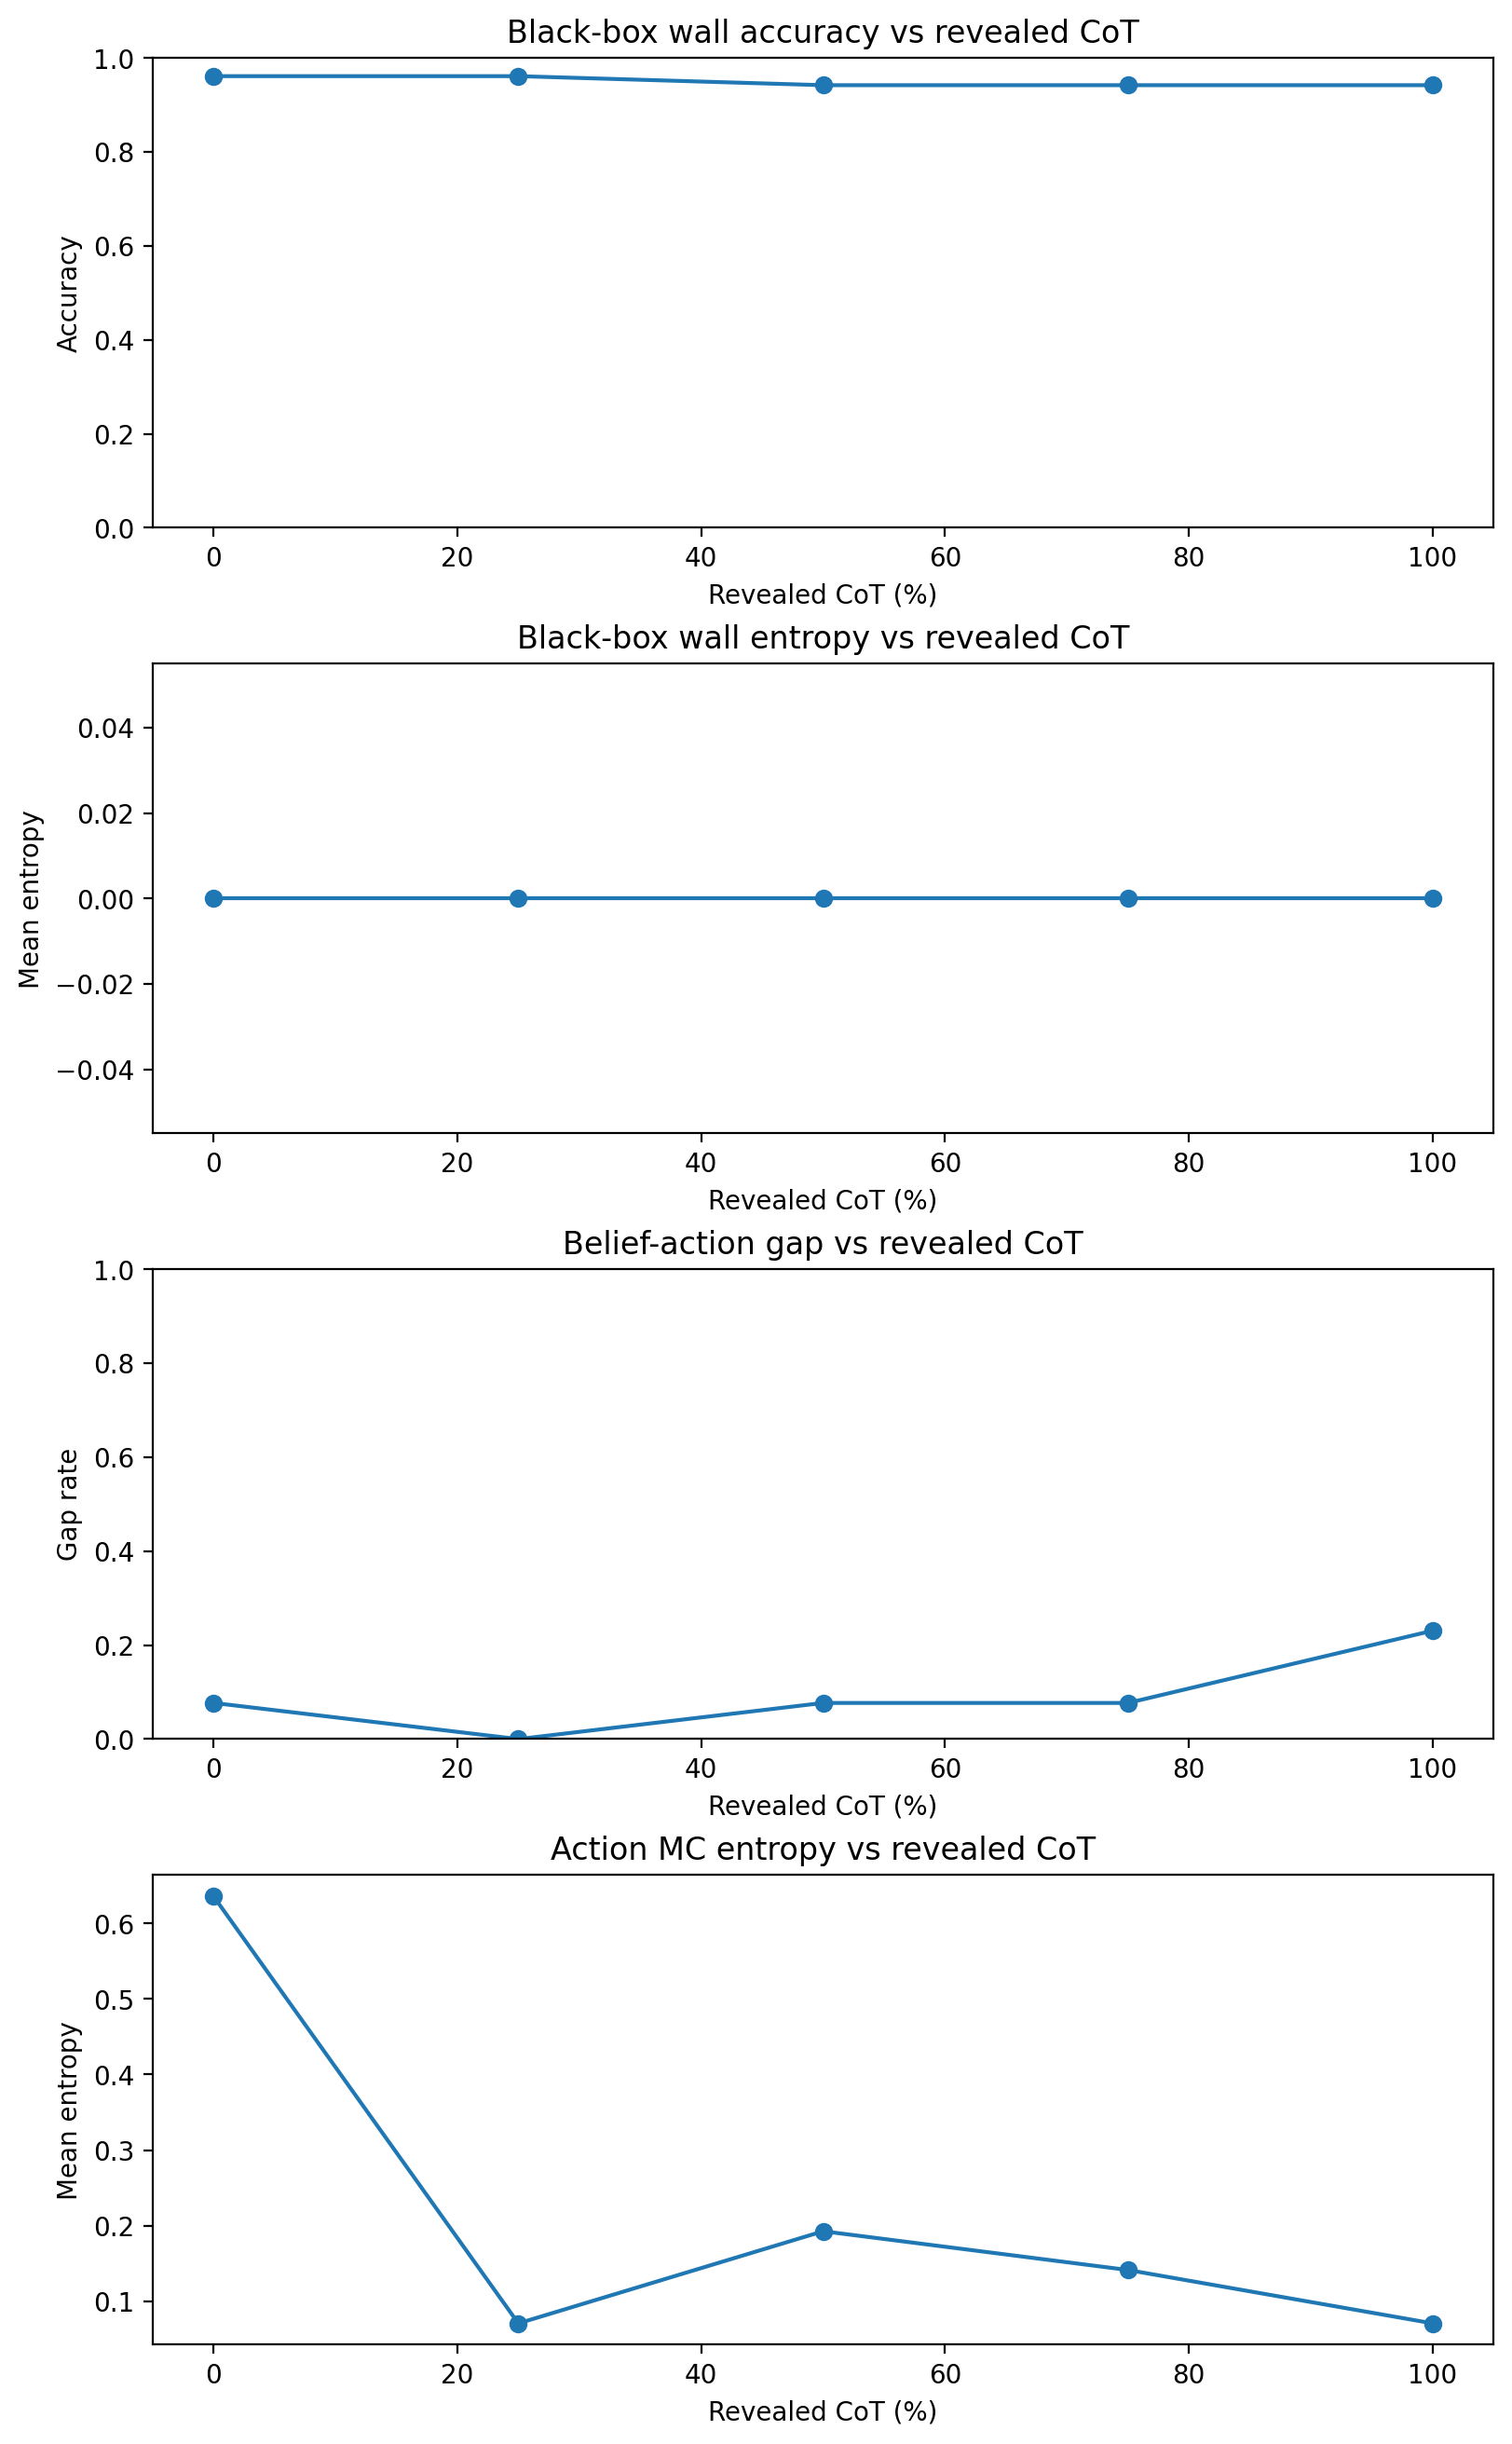
\includegraphics[width=0.8\linewidth]{figs/gradual_blackbox_reasoning_failure.png}
    \caption{Behavioural effects of gradually revealing prior chain-of-thought on a failure-focused slice. Wall-belief accuracy remains high and wall-label entropy remains near zero across reveal levels, while MC-sampled action entropy decreases and belief-action gap rates increase with reveal level.}
    \label{fig:gradual_cot_blackbox_full}
\end{figure}



\subsection{Four-Room Episode Sweep: Optimal Geometry vs Agent Action Bias}

The four-room experiment compares two label choices while holding activations, architecture, and training procedure fixed. Model A is trained on the agent's emitted actions; Model B is trained on full-state BFS-optimal actions.

\begin{table}[h]
\centering
\begin{tabular}{lrr}
\toprule
Metric & Agent-action label & BFS-optimal label \\
\midrule
Test accuracy & 0.454 & \textbf{0.960} \\
Test set-membership accuracy & 0.369 & \textbf{0.992} \\
Test log-likelihood & $-0.9969$ & \textbf{$-0.1389$} \\
Train accuracy & 0.451 & \textbf{0.972} \\
Majority-class baseline & 0.548 (UP) & 0.733 (DOWN) \\
Random baseline & 0.250 & 0.250 \\
\bottomrule
\end{tabular}
\caption{Four-room label-control result. Identical activations and algorithm; only the label changes.}
\label{tab:fourroom-main}
\end{table}

\begin{result}
The same activation features predict full-state BFS-optimal actions at 96.0\% accuracy and 99.2\% optimal-set membership, but predict the agent's own actions only 45.4\%, below the majority baseline. This shows that the activation representation is much more predictive of optimal geometry than of the agent's behavioural UP-bias.
\end{result}

\paragraph{Pre/post clarification.} In the four-room experiment, pre- and post-reasoning state features are tied for optimal-label prediction because $\phi(s)$ is visit-averaged over all visits to the same state. Averaging removes trajectory-specific output-commitment information and preserves stable state geometry. This does not contradict per-visit pre/post dissociation; the two experiments answer different questions.


\section{Limitations}

The main limitation is causal: probe success indicates decodability, not causal use.
A probe can reveal that information is present in an activation space without proving
that the model uses that information to generate its action. 
A second limitation is environment simplicity. DoorKey is useful for exact analysis
because the true state, transition function, and optimal-action set are all computable.
However, the environment is small enough that the agent may be near-ceiling on many
states even without internalising a coherent value function, and the results may not
generalise to richer environments with larger state spaces or longer horizons.
All experiments use a single model (GPT-OSS-20B); it is unknown whether the
belief-degradation pattern across reasoning holds for other models or training regimes.
The current behavioural results establish two separate findings: exact-state agreement between representational and behavioural wall probes on a limited public clean slice, and a behavioural-only failure-focused revealed-CoT analysis showing that increased reasoning reveal does not reduce the measured gap. The next stage is to join failure-focused behavioural probes, white-box probes, emitted actions, and IRL/value predictions on the same states. Distributional optimal-action metrics are needed for tied optimal actions, and causal patching is needed to test whether decoded representations influence later reasoning and final action generation. If these analyses support the current pattern, the project will provide a concrete methodology for moving from behavioural evaluation to mechanistic diagnosis of LLM-agent failures.

\section{Conclusion}

This project asks whether language-model agents fail because they lack task-relevant information, or because they fail to use information already available in their internal representations. The evidence supports the second explanation. Across experiments, pre-reasoning activations encode task-optimal actions far more reliably than the agent’s final behavior: layer-15 probes recover optimal actions at 97.6\% on the fixed grid, 96.0\% in the four-room sweep, and 79.3\% on the stricter Seed12 evaluation, while the agent acts optimally only 58.7\%, 32.5\%, and 12.7\% of the time in those same settings. Thus, the decodable-action versus enacted-action gap ranges from 39 to 67 percentage points.

The chain-of-thought process appears to close this gap, but by committing the model to an action rather than by simply revealing better beliefs. From pre- to post-reasoning, the belief-action gap $\Delta_t$ decreases significantly across all four evaluation subsets, while state entropy $H_t$ increases ($p < 0.0001$). The causal experiment $f(X_1, R_2)=Y_{12}$ shows that the reasoning trace, rather than the input-state representation, determines the final action: $Y_{12}=Y_2$ in 100\% of cases, with a 76\% flip rate. By contrast, interventions on pre-reasoning activations alone have no detectable effect. These results support a routing account: task-relevant information is present before reasoning, but the reasoning process redirects the model toward an action commitment that can depart from that information.

The steering results sharpen this account. The corrected verbose-prompt flag-swap experiment shows that the layer-15 suffix representation is not directly read out by the action head. Causal control only appears when the intervention matches the relevant layer, prompt format, and baseline action direction. This suggests that belief-to-action causality depends on whether the representation lies on the action-generation pathway used by that specific prompt format.

Behavioral probes show that the gap is not merely a probe artefact. In wall-hit cases, the model can correctly state that its chosen direction is blocked and still take that action. White-box and black-box wall probes agree at 73--100\% across directions on the matched public slice, indicating that both methods identify similar state information. Cases where both probes show correct knowledge but the emitted action remains wrong provide the strongest evidence for action-selection failure rather than belief failure.

The next stage should align all measurement streams at the state level: representational probes, behavioral probes, IRL predictions, and emitted actions. This will allow each failure to be classified as a belief failure, routing failure, or value-misalignment failure. The analysis should also probe intermediate reasoning-token positions to locate where the optimal-action signal is lost and where action commitment emerges. Finally, bidirectional causal patching should test whether injecting pre-reasoning belief activations into post-reasoning positions can repair wrong actions, and whether post-reasoning commitments can override correct beliefs.

\bibliographystyle{plain}
\bibliography{refs}

\clearpage
\appendix
\section{Behavioural Probe Appendices}

\subsection{Behavioural Probe Prompts}
The behavioural probes use a shared instruction scaffold: the same environment description, legend, directional conventions, and answer-format constraints. The probed object or relation changes, not the scaffold.

\paragraph{Canonical wall prompt (semantic label path).}
\begin{verbatim}
# Instructions

You are controlling an agent in a 9x9 fully observable DoorKey GridWorld.
The environment contains walls, open spaces, a goal, a key, and doors.

Legend:
---------------
#: Wall
_: Open Space
G: Goal
A: Current agent position
D: Door (closed/locked)
O: Door (open)
K: Key
---------------

Interpret RIGHT as the cell one column to the right (east), LEFT as the
cell one column to the left (west), UP as one row up (north), and DOWN as
one row down (south) in the rendered grid.

# Inputs

Current grid state:

  0 1 2 3 4 5 6
0 # # # # # # #
1 # _ _ _ _ _ #
2 # A _ _ _ _ #
3 # _ _ _ _ _ #
4 # _ _ _ G _ #
5 # _ _ _ _ _ #
6 # # # # # # #

Agent status:
- Carrying key: false

Given the current grid only, is the cell immediately RIGHT of the agent a
wall (#)?

Return exactly one label and nothing else:
A = yes
B = no
C = unknown
\end{verbatim}

\paragraph{Wall prompt variant (JSON sampled-answer path).}
\begin{verbatim}
Return exactly one JSON object of the form
{"label": "<yes|no|unknown>"} and nothing else.
\end{verbatim}

\paragraph{Canonical action prompt.}
\begin{verbatim}
# Instructions

You are controlling an agent in a 9x9 fully observable DoorKey GridWorld.
The environment contains walls, open spaces, a goal, a key, and doors.

Legend:
---------------
#: Wall
_: Open Space
G: Goal
A: Current agent position
D: Door (closed/locked)
O: Door (open)
K: Key
---------------

Interpret RIGHT as the cell one column to the right (east), LEFT as the
cell one column to the left (west), UP as one row up (north), and DOWN as
one row down (south) in the rendered grid.

Choose the next move that best advances toward the goal while respecting
the DoorKey mechanics in the current state.

The key is automatically picked up when the agent moves onto K. A closed
door D can only be opened if the agent already has the key.

# Inputs

Current grid state:

  0 1 2 3 4 5 6
0 # # # # # # #
1 # _ _ _ _ _ #
2 # A _ _ _ _ #
3 # _ _ _ _ _ #
4 # _ _ _ G _ #
5 # _ _ _ _ _ #
6 # # # # # # #

Respond with exactly a JSON object of the form
{"action": "<UP|DOWN|LEFT|RIGHT>"}.
Do not include any extra text before or after the JSON.
\end{verbatim}

\paragraph{Revealed-CoT action prompt variant.}
\begin{verbatim}
Reasoning trace available so far:
We need shortest path from A at (2,1) to G at (4,4). Grid open spaces.
Likely move down two then right three. But check walls: row4 col4 is G.
Path: from (2,1) down to
\end{verbatim}

\subsection{Prompt Variants}
The same base prompt scaffold is used across wall, key, door, and location probes where applicable. Variants are limited to the target object or relation, the answer format, and the optional revealed-CoT block. Repeated greedy and Monte Carlo readouts differ in sampling regime rather than semantic task definition.

\subsection{Selected Failure Cases}
Figure~\ref{fig:wall_hit_suboptimality_cases_full} shows concrete wall-hit and sub-optimality cases in which the model reports the local wall fact correctly yet still takes a wall-hitting or non-optimal action.

\begin{figure}[h]
    \centering
    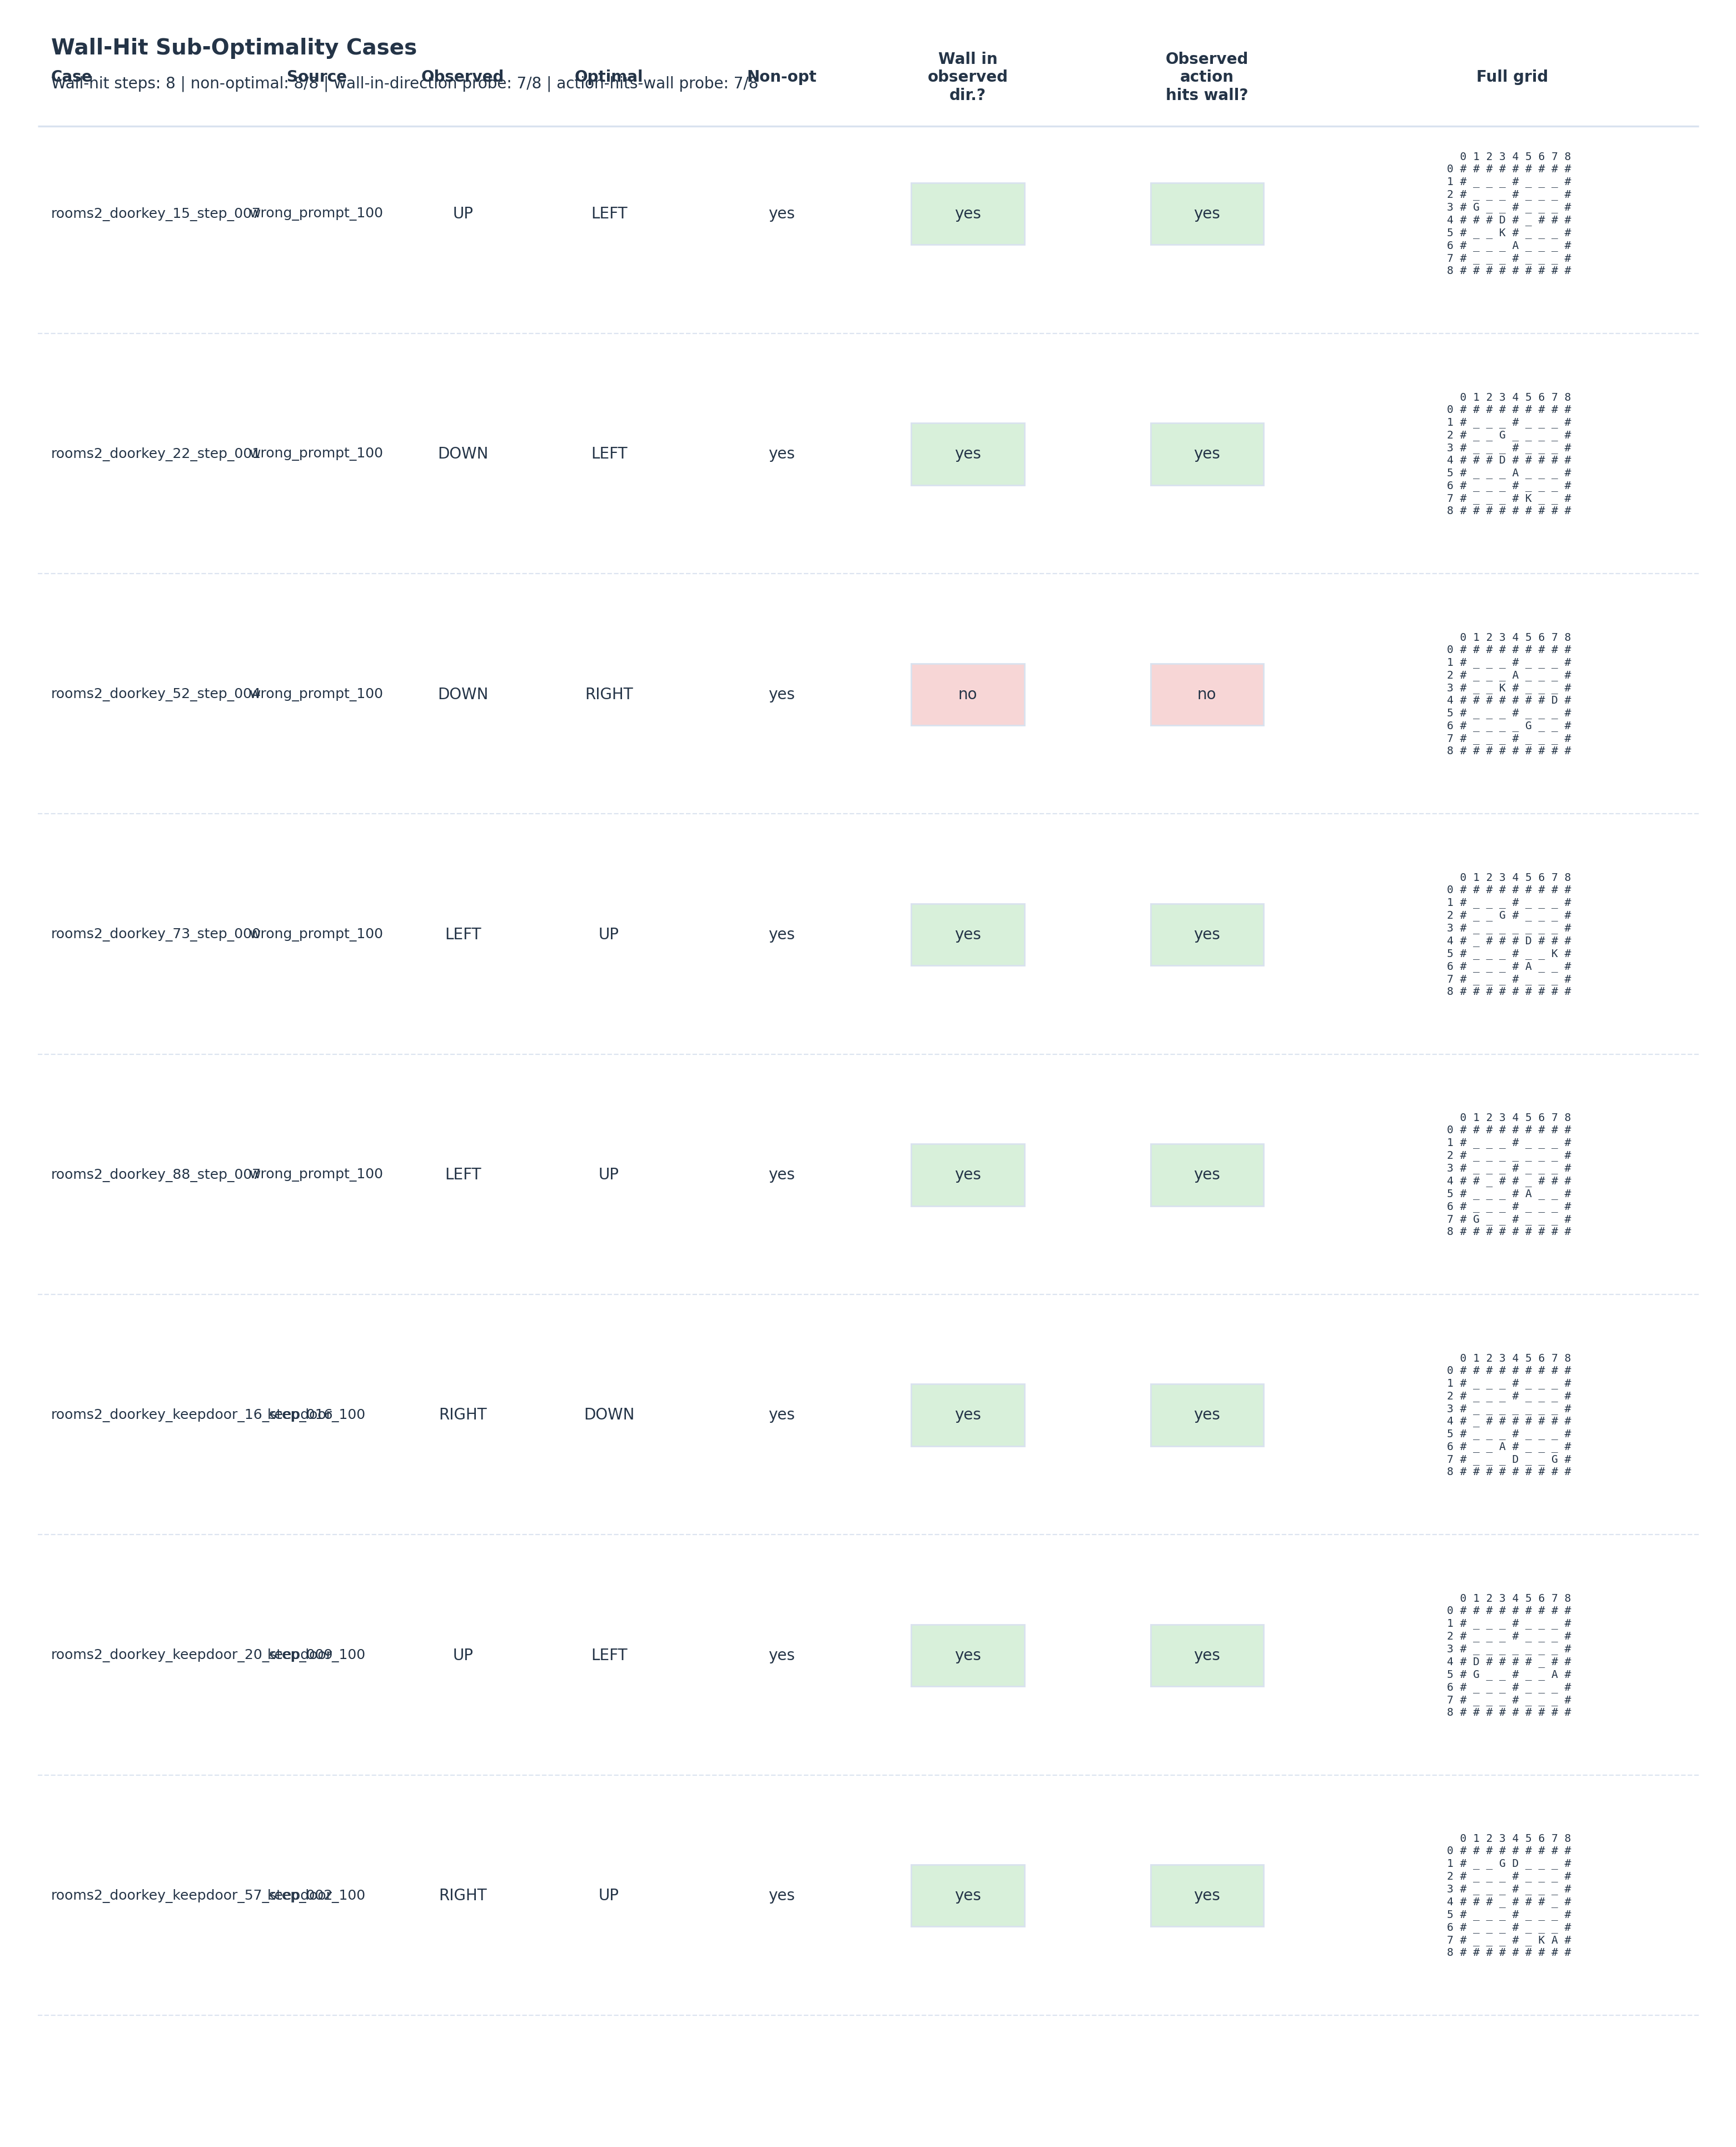
\includegraphics[width=\linewidth]{figs/wall_hit_suboptimality_cases.png}
    \caption{Selected wall-hit and sub-optimality cases from the behavioural failure analysis.}
    \label{fig:wall_hit_suboptimality_cases_full}
\end{figure}

\subsection{Additional Behavioural Figures}

\begin{figure}[h]
    \centering
    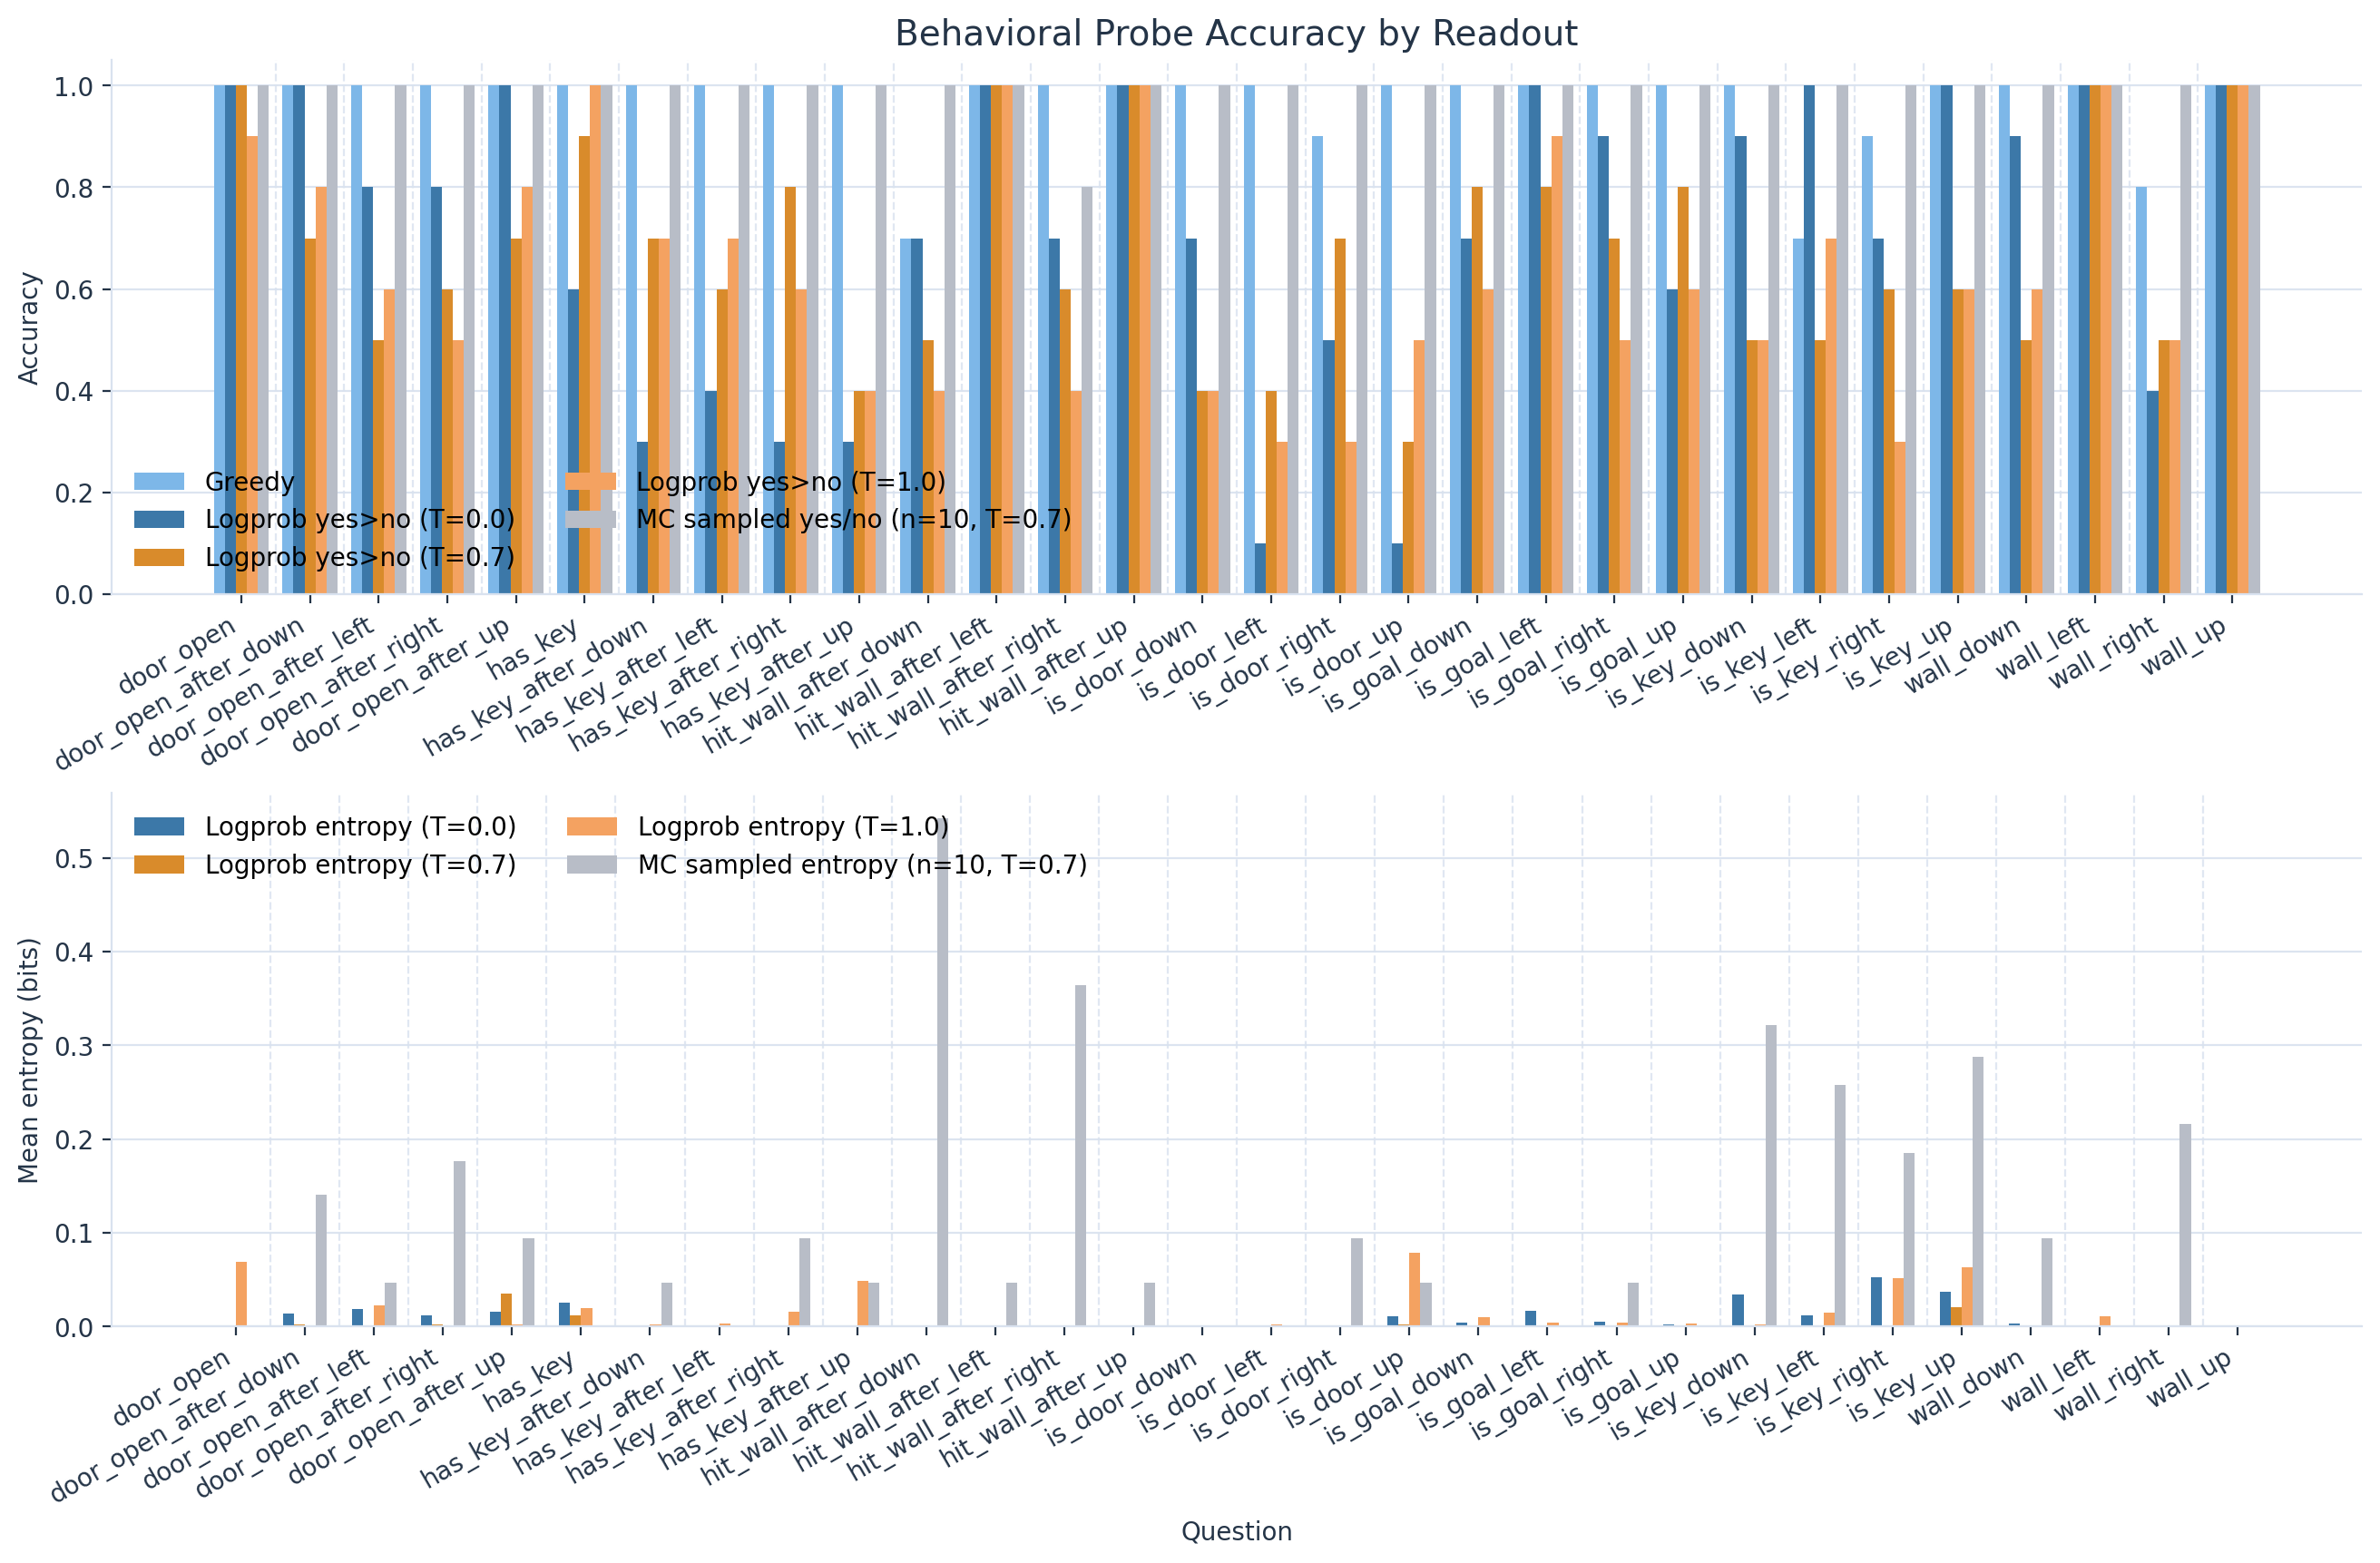
\includegraphics[width=\linewidth]{figs/behavioral_probe_summary_overview_appendix.png}
    \caption{Broad behavioural probe summary on the smoke-test-all suite.}
\end{figure}

\begin{figure}[h]
    \centering
    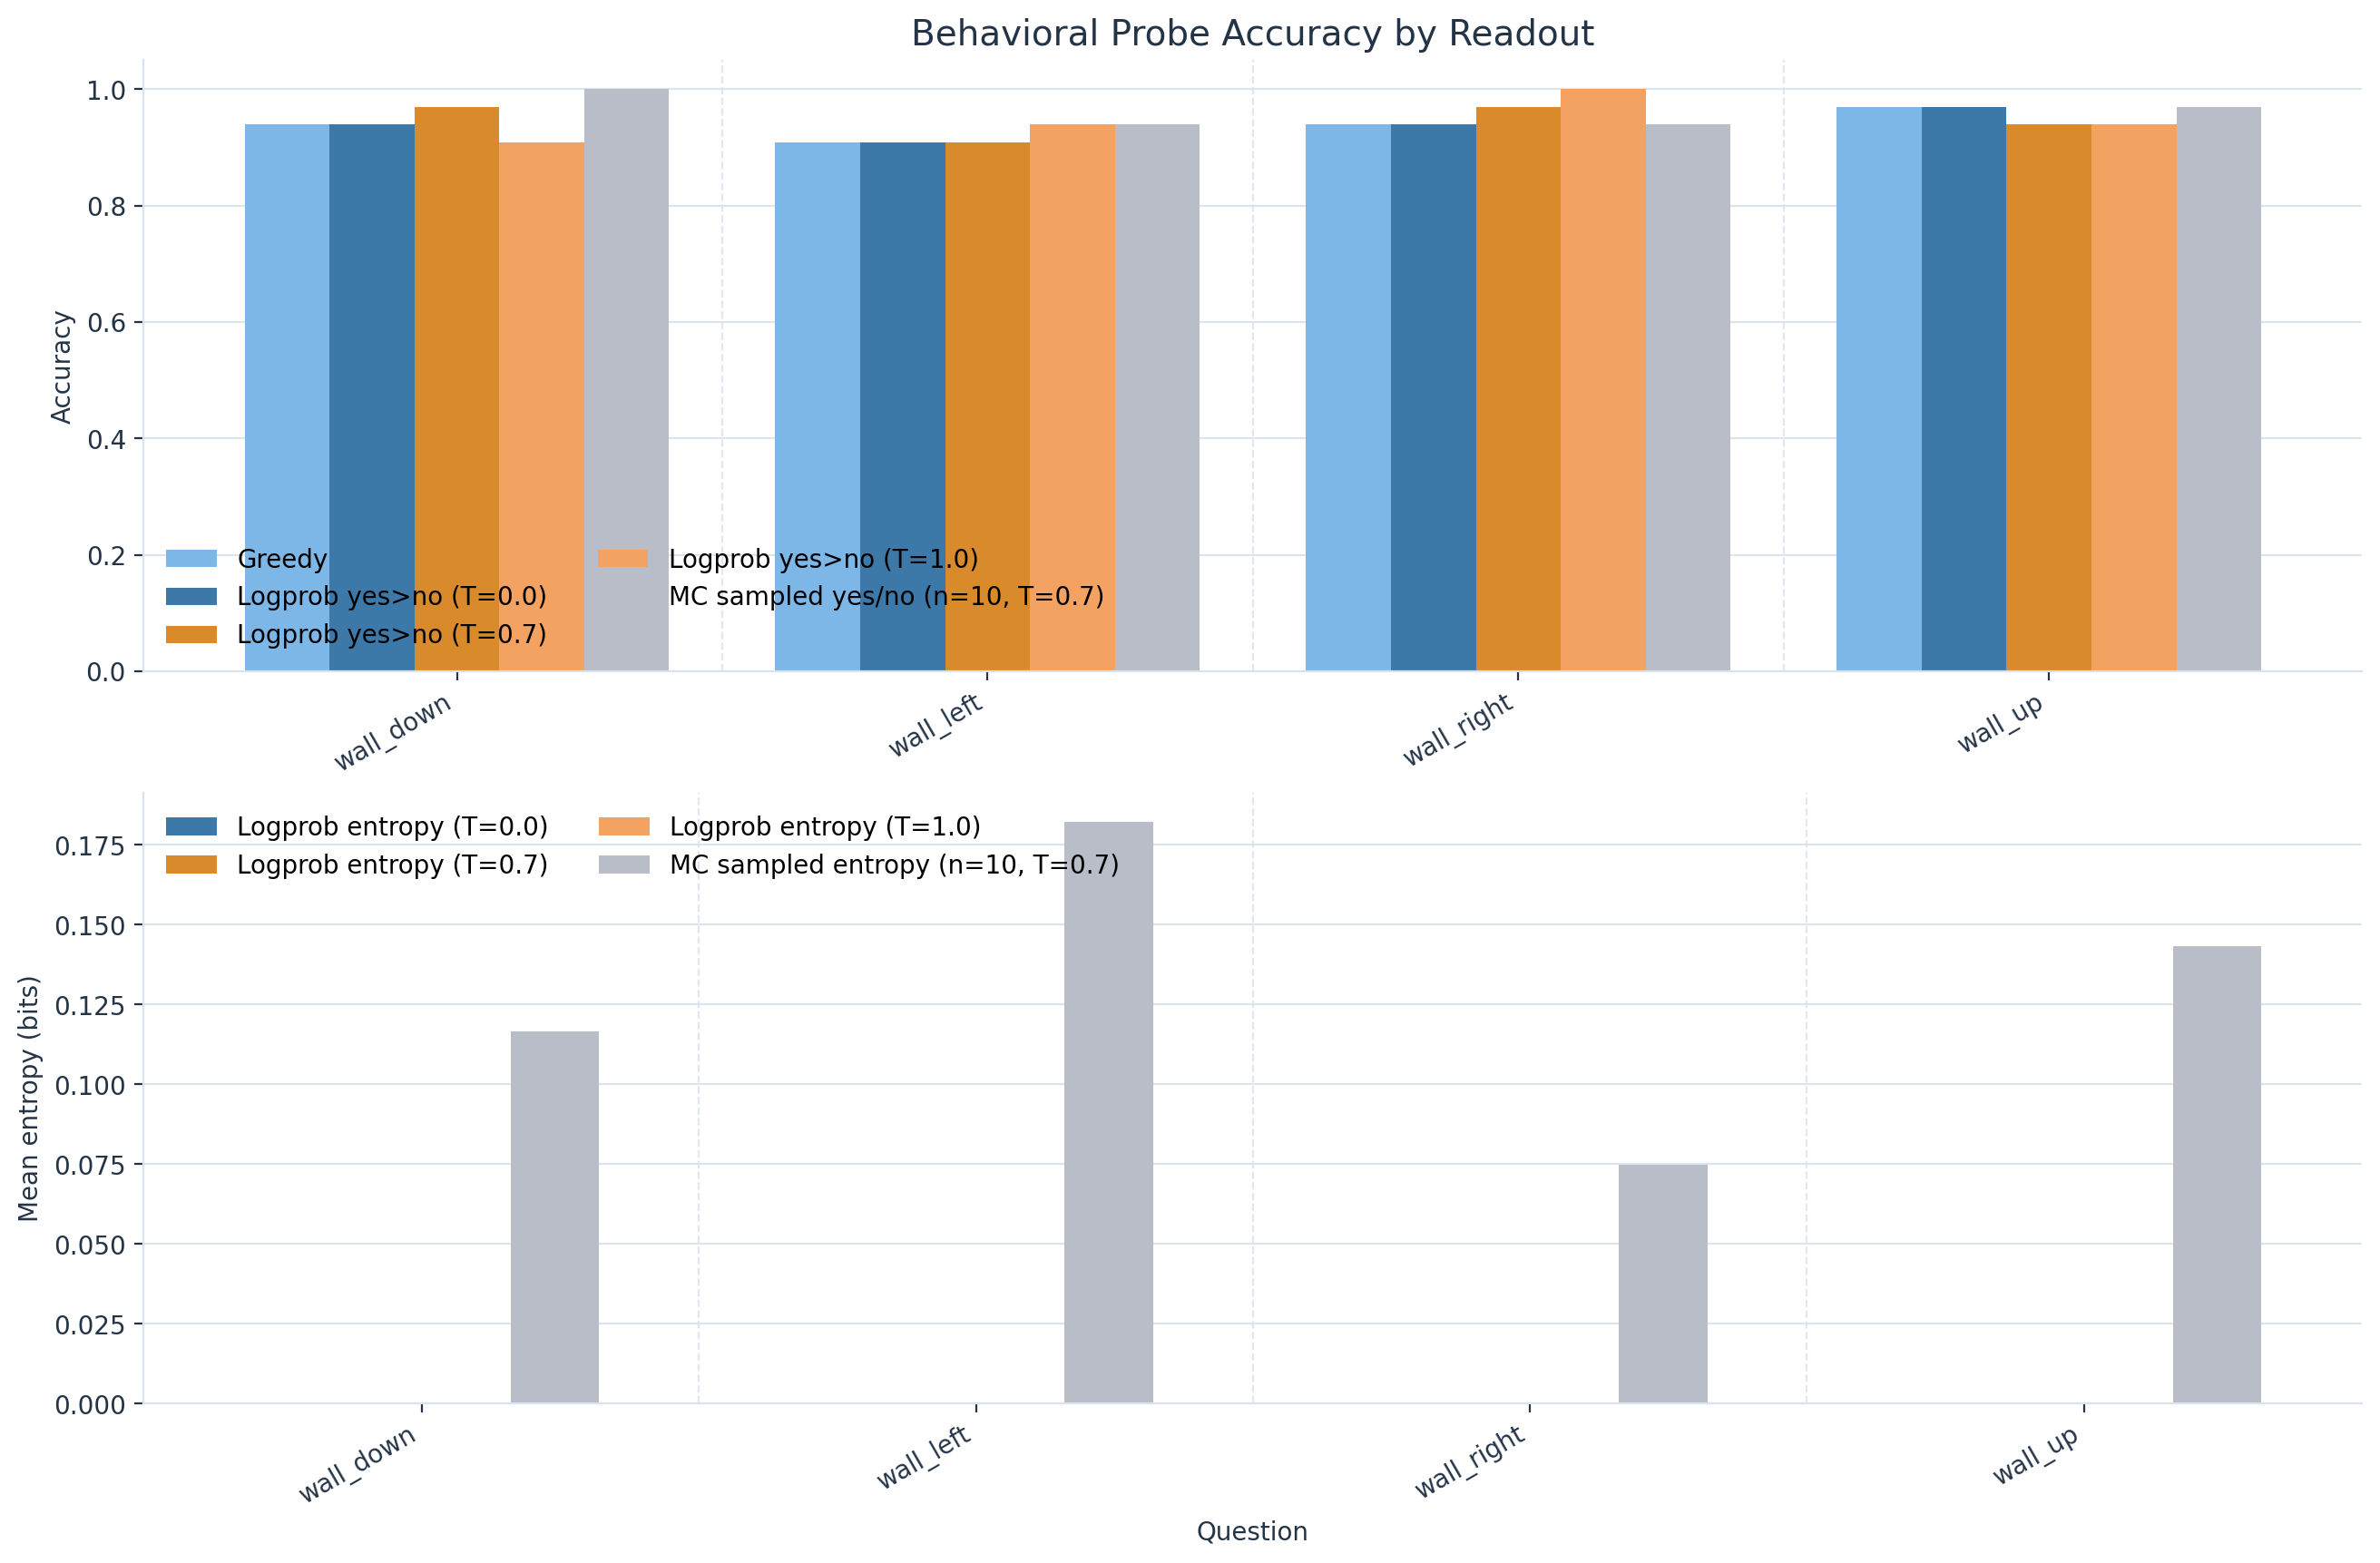
\includegraphics[width=\linewidth]{figs/behavioral_probe_summary_wall_gap_appendix.png}
    \caption{Wall-focused behavioural probe summary on the failure slice.}
\end{figure}

\end{document}
